\documentclass[12pt,a4paper]{article}

% ── Encoding & fonts ──────────────────────────────────────────────────────────
\usepackage[T1]{fontenc}
\usepackage[utf8]{inputenc}
\usepackage{lmodern}
\usepackage{microtype}

% ── Page geometry ─────────────────────────────────────────────────────────────
\usepackage[a4paper,
            top=2.5cm, bottom=2.5cm,
            left=2.8cm, right=2.8cm,
            headheight=14pt]{geometry}

% ── Line spacing ──────────────────────────────────────────────────────────────
\usepackage{setspace}
\setstretch{1.15}

% ── Colours ───────────────────────────────────────────────────────────────────
\usepackage[dvipsnames,table]{xcolor}
\definecolor{accent}{RGB}{30,80,130}
\definecolor{tablehead}{RGB}{220,230,242}

% ── Headings & sections ───────────────────────────────────────────────────────
\usepackage{titlesec}
\titleformat{\section}{\large\bfseries\color{accent}}{{\thesection.}}{0.6em}{}[\vspace{-0.3ex}\color{accent}\hrule height 0.4pt\vspace{0.3ex}]
\titleformat{\subsection}{\normalsize\bfseries\color{accent}}{{\thesubsection}}{0.5em}{}
\titlespacing*{\section}{0pt}{1.4em}{0.5em}
\titlespacing*{\subsection}{0pt}{1em}{0.3em}

% ── Headers & footers ─────────────────────────────────────────────────────────
\usepackage{fancyhdr}
\pagestyle{fancy}
\fancyhf{}
\renewcommand{\headrulewidth}{0.4pt}
\fancyhead[L]{\small\color{gray}McKern \textbar\ NeuralNations Working Papers}
\fancyhead[R]{\small\color{gray}May 2026}
\fancyfoot[C]{\small\thepage}

% ── Tables ────────────────────────────────────────────────────────────────────
\usepackage{booktabs}
\usepackage{tabularx}
\usepackage{array}

% ── Lists ─────────────────────────────────────────────────────────────────────
\usepackage{enumitem}
\setlist[itemize]{leftmargin=1.5em, itemsep=0.2em, topsep=0.4em}

% ── Hyperlinks ────────────────────────────────────────────────────────────────
\usepackage[colorlinks=true,
            linkcolor=accent,
            citecolor=accent,
            urlcolor=accent,
            pdfauthor={Kari Freyr McKern},
            pdftitle={A Functional Taxonomy of Human Social Organisation},
            pdfsubject={CAMS framework; coordination theory; civilisational taxonomy},
            pdfkeywords={CAMS, coordination, taxonomy, complexity, institutions}
            ]{hyperref}

% ── Abstract box ──────────────────────────────────────────────────────────────
\usepackage{mdframed}
\mdfsetup{
  innerleftmargin=14pt,
  innerrightmargin=14pt,
  innertopmargin=10pt,
  innerbottommargin=10pt,
  linecolor=accent,
  linewidth=1pt,
  backgroundcolor=tablehead
}

% ── Misc ──────────────────────────────────────────────────────────────────────
\usepackage{parskip}
\setlength{\parskip}{0.55em}
\setlength{\parindent}{0pt}
\usepackage{datetime2}
\usepackage{graphicx}

% ─────────────────────────────────────────────────────────────────────────────
%  DOCUMENT
% ─────────────────────────────────────────────────────────────────────────────
\begin{document}

% ── Title block ───────────────────────────────────────────────────────────────
\begin{center}
  {\LARGE\bfseries\color{accent} A Functional Taxonomy of Human\\[0.3ex] Social Organisation}\\[1.2em]
  {\large\itshape Coordination Problems, Geography, and the\\
  Eight-Node Architecture of Human Meta-Systems}\\[1.4em]
  {\normalsize\textbf{Kari Freyr McKern}}\\[0.3em]
  {\small Independent Researcher, Sydney, Australia}\\[0.2em]
  {\small \href{https://neuralnations.org}{neuralnations.org} \quad$\cdot$\quad May 2026}\\[0.5em]
  {\small\color{gray} NeuralNations Working Paper~3 (v3)}
\end{center}

\vspace{1em}
\begin{mdframed}
\textbf{Abstract}\\[0.5em]
This paper proposes a formal taxonomy of social coordination architectures grounded in the Complex Adaptive Model State (CAMS) framework. The taxonomy is built from below rather than imposed from above. It begins with the eight recurring coordination problems that any sufficiently differentiated Holocene human society must solve, identifies how geography makes some of these problems acute and others latent, and shows how local solutions accumulate into path-locked institutional architectures. The eight CAMS nodes---Helm, Shield, Lore, Stewards, Craft, Hands, Archive, Flow---are then warranted as the minimal functional decomposition at which the recurring coordination problems become surveyable: not as an arbitrary social-science taxonomy but as one node per recurring problem. Empirical clustering across 229 polities recovers eight stable groupings without geographic priors, including durable structural similarities between Rome, the Ottoman Empire, the Yuan Dynasty, the British Empire, and the People's Republic of China. The taxonomy is offered as evidence that coordination architecture, not regime type or development stage, is the relevant axis along which human meta-systems differ. The formal mechanism of path dependency itself---the Library Attractor---is developed in a companion paper~\cite{mckern2026library}.

\medskip
All datasets, scoring protocols, dendrograms, and reproducible code are available at \href{https://neuralnations.org}{neuralnations.org} and \href{https://github.com/KaliBond/wintermute}{github.com/KaliBond/wintermute}.
\end{mdframed}

\vspace{1em}
\hrule height 0.5pt
\vspace{0.5em}

% ─────────────────────────────────────────────────────────────────────────────
\section{Introduction}
% ─────────────────────────────────────────────────────────────────────────────

The taxonomic question in social science has been treated, for several decades, as a methodological liability. To classify societies risked reifying ideological categories---modern and traditional, Western and non-Western, advanced and primitive---that revealed more about the classifier than about the classified. The discipline retreated, for good reasons, towards either case-specific historical analysis or universal-mechanism theorising, leaving comparative typology to a small literature whose ambitions outran its evidentiary base.

This retreat has costs. Without a taxonomy, claims about why some societies persist while others collapse, why coordination problems recur in similar forms across millennia, or why institutional configurations cluster in geographically interpretable ways, all remain narrative. They cannot be falsified, replicated, or aggregated.

The argument of this paper is that the taxonomic question can now be answered formally and falsifiably, provided it is framed correctly. The wrong starting point is \textit{types of society}, which immediately invites ideological framing. The right starting point is \textit{types of coordination problem}, which are imposed by ecology and scale rather than chosen by analysts. If we can identify the recurring coordination problems that Holocene human societies face, observe that geography makes some of those problems acute in particular regions, watch how local solutions accumulate into institutional architectures, and demonstrate that the resulting architectures cluster empirically, then the taxonomy follows from the evidence rather than being projected onto it.

This paper makes that argument in seven steps. Section~2 sets out the eight recurring coordination problems. Section~3 shows how geography poses these problems differentially across ecological zones. Section~4 introduces the path-dependency claim that turns local solutions into civilisational architectures. Section~5 warrants the eight-node CAMS grammar as the minimal functional decomposition at which the coordination problems become surveyable, addressing the question ``why eight?''. Section~6 presents the empirical taxonomy that emerges from hierarchical clustering across 229 polities. Section~7 discusses the placements that resist conventional framings of the United States, the People's Republic of China, and the Russian Federation. Section~8 sets out falsifiability conditions specific to the taxonomic claim.

The companion paper~\cite{mckern2026library} develops the formal operator of path dependency---the Library Attractor---that the taxonomy implies. Earlier papers establish the framework's foundations~\cite{mckern2026paper1} and the diagnostic phase space.

% ─────────────────────────────────────────────────────────────────────────────
\section{The Eight Recurring Coordination Problems}
% ─────────────────────────────────────────────────────────────────────────────

A useful taxonomy of human meta-systems begins with the problems they all have to solve. The following eight have been recurrently distinguishable in differentiated Holocene societies; they are stable across scale, technology, and historical era because each corresponds to a functional pressure that does not disappear when its current institutional solution is replaced by another.

\begin{enumerate}[leftmargin=1.8em, label=\textbf{\arabic*.}]

\item \textbf{Direction under uncertainty.} Who decides what to do when futures are uncertain, when the time-pressure of decision exceeds the time-pressure of consensus, and when distributed information cannot be aggregated quickly enough by ordinary deliberation? This problem is universal because environmental, adversarial, and demographic uncertainty are universal. It can be solved by a chief, a council, a constitutional executive, an algorithm, or a junta---but it has to be solved.

\item \textbf{Boundary maintenance.} How is the system protected from external predation, internal violence, and definitional dissolution? This is not only a military problem; it is the problem of selective porosity---what gets in, who stays in, what stays out. It can be solved by walls, navies, oaths of allegiance, citizenship law, or border officers, but the function recurs at every scale.

\item \textbf{Meaning integration.} What gives the system coherent sense to its members? What turns a collection of individuals in geographic proximity into an \textit{us} who can sustain coordinated action across generations? This problem becomes acute as scale increases and personal acquaintance can no longer carry the integrative work. Religion, ideology, civic ritual, education, and shared narrative are all candidate solutions.

\item \textbf{Allocation.} Who owns what, who gets what, and by what rule? This problem becomes acute once surplus exists. It involves not only the immediate distribution of resources but the rules under which property, rents, taxes, and obligations are transmitted across generations. Property regimes, fiscal systems, gift economies, and centralised redistribution are all candidate solutions.

\item \textbf{Technical reproduction.} How is technical knowledge---agricultural, metallurgical, navigational, military, medical, administrative, scientific---preserved across generations and applied to material problems? This problem requires apprenticeships, schools, guilds, professional bodies, or research institutions, but the function is invariant: technique is fragile, and a society that cannot reproduce its technical base loses material capacity within a generation.

\item \textbf{Labour reproduction.} How is the population that does the work reproduced---not only biologically but institutionally? Who learns to be a farmer, a soldier, a scribe, a nurse? This problem requires fertility regimes, household structures, kinship rules, migration policies, and labour-market institutions. It is not the same problem as technical reproduction; the institutional infrastructure for raising and placing people differs from the infrastructure for transmitting skills.

\item \textbf{Memory.} How is precedent stored, retrieved, and applied to current decisions? How do current decisions take into account decisions made before living memory? This problem requires archives, law, historiography, bureaucracy, and writing in the technical sense. Without an answer to this problem, every generation rediscovers the same lessons by paying the same costs.

\item \textbf{Circulation.} How do goods, information, persons, and services move within and across the system's boundary? This problem requires roads, ports, postal systems, currencies, markets, contract law, and now electronic networks. The function is not the same as production or possession; it is the moving of what is produced and possessed to where it is wanted, and the integration of distant production into local consumption.

\end{enumerate}

These eight problems are not a list of social subsystems. They are a list of recurring functional pressures. A society's institutional architecture is its accumulated set of solutions to these pressures, and two societies with very different institutional architectures may both be recognisably solving the same problem with different means. The Yuan Dynasty, the Ottoman Empire, and the Republic of Venice all solved the eight problems; their solutions diverged radically; the problems were the same.

The argument of this paper is that taking the problems as primary and the institutions as derivative is the move that makes a non-ideological taxonomy possible.

% ─────────────────────────────────────────────────────────────────────────────
\section{Geography as Problem-Poser}
% ─────────────────────────────────────────────────────────────────────────────

Geography does not determine social outcomes. It does, however, determine which of the eight coordination problems are \textit{acute} in a given environment and which are \textit{latent}. The same set of problems is everywhere in the background, but the relative pressure varies dramatically with ecology. Different ecological zones therefore select for different relative weightings of the institutional solution-set, and over centuries those weightings accumulate into recognisable civilisational morphologies.

\textbf{Riverine ecologies}---the Tigris-Euphrates, the Nile, the Indus, the Yellow River, the Mekong floodplain---make \textit{Allocation} and \textit{Memory} acute. Annual flooding cycles require multi-year planning, water-rights adjudication, granary management, and the calendrical predictions that follow from systematic record-keeping. Mesopotamian, Pharaonic, and early Chinese coordination architectures all converged on bureaucratic Stewards--Archive primacy because the problem-set demanded it.

\textbf{Maritime trade ecologies}---the Mediterranean, the Baltic and North Sea, the Indian Ocean rim, the South China Sea archipelagos, the North Atlantic---make \textit{Circulation} and \textit{Direction under uncertainty} acute. Trade networks reward fast-loop adaptation; long voyages require executive authority that can act without continuous reference to a central capital. The Phoenician city-states, classical Athens, the Italian maritime republics, the Hanseatic League, and the Dutch Republic converged on Flow--Helm primacy with weaker Archive coupling because the problem-set rewarded it.

\textbf{Continental ecologies}---the great Eurasian heartland, central North America before continental settlement, central Africa above the rainforest line---make \textit{Boundary maintenance} and \textit{Direction} acute. Without natural barriers, defence is everywhere a present problem; legitimacy must travel further than it can be enforced. Continental polities therefore tend towards Shield--Helm primacy with Archive playing a strong supportive role. The Achaemenid Empire, the Mongol Empire, the Russian Empire, and the contemporary Russian Federation are all recognisable as continental coordination architectures despite vast differences in technology and ideology.

\textbf{Mountain ecologies}---the Andes, the Tibetan Plateau, the Caucasus, the Alpine zones---make \textit{Allocation} (across vertical production zones) and \textit{Meaning integration} acute. Vertical zonation produces multiple specialised production environments within short horizontal distances; small populations require high internal cohesion to maintain social viability. The Inca, Tibetan, Andean, and Caucasian polities therefore tend towards Stewards--Lore primacy.

\textbf{Steppe and pastoral ecologies}---the Eurasian steppe, the Sahel, the Arabian peninsula before urbanisation---make \textit{Boundary maintenance} and \textit{Labour reproduction} acute in a particular form: the population is mobile, herds are the resource base, and military pressure is constant. Archive is structurally weak because writing is costly when the polity is literally on the move; Flow is strong because mobility is the default. Mongol, Turkic, Scythian, and pre-imperial Arabian coordination architectures share these features despite their independent histories.

\textbf{Insular ecologies}---Japan, Britain, Sri Lanka, Madagascar, the larger Pacific islands---make \textit{Boundary maintenance} trivial (geography solves it) but \textit{Circulation} particularly important (the external interface is concentrated). Archive and Lore can be strong because membership is bounded by sea; Flow becomes the dominant external function. Tokugawa Japan, pre-industrial Britain, and the larger insular polities of the Indian Ocean rim show recognisable Archive--Flow signatures.

\textbf{Tropical forest ecologies}---Amazonia, the Congo basin, the older interior of Southeast Asia---make centralisation costly. Dispersion of population, difficulty of long-distance Circulation, and the relative ease of horizontal exit all militate against single-centre solutions to the eight problems.

These are tendencies, not laws. The point is not that geography assigns morphology deterministically; the point is that geography poses problems differentially, and the differential problem-pressure selects for differential institutional weighting.

% ─────────────────────────────────────────────────────────────────────────────
\section{Path Dependency: How Local Solutions Become Civilisational Architectures}
% ─────────────────────────────────────────────────────────────────────────────

Once a configuration succeeds at solving the local problem-set well enough to produce surplus and reproduce itself across generations, three mechanisms drive its consolidation into a civilisational architecture.

\textbf{Capacity accumulation.} Each generation that operates the configuration improves the institutional capacity associated with the privileged nodes. A bureaucratic riverine state develops more sophisticated Archive practices over time; a maritime trade republic develops more elaborate Flow protocols. The accumulated capacity becomes a sunk asset that is costly to discard.

\textbf{Bond strength formation.} The functional links between nodes---the ways in which Helm and Stewards work together, in which Archive feeds Lore, in which Shield protects Flow---accumulate operating routines that are not separately specified but emerge from repeated use. A society can in principle copy another's institutions but it cannot copy their bond structure, which is the residue of generations of working interaction.

\textbf{Solution-by-extension.} New problems, when they emerge, get addressed using the existing architecture rather than by reorganising it. The riverine bureaucracy responds to a new technology by integrating it through Stewards and Archive; the maritime trade republic responds to a new technology by integrating it through Flow and Helm. Each successful application of the existing architecture to a new problem reinforces the architecture's status as the default way of solving problems in that society.

The combined effect is \textit{morphological lock-in}. After sufficient time, the configuration becomes the tacit assumption about how things work. Departing from it requires not only finding an alternative that works but overcoming the accumulated capacity, bond structure, and habitual problem-solving routines of the existing architecture.

This is path dependency in the strict sense~\cite{pierson2000}. It is not a claim that history determines outcomes deterministically; it is a claim that the cost of leaving an established morphology rises with time of occupation, and that under most conditions the existing morphology is preserved against shocks rather than replaced.

The formal mechanism---what determines when path dependency holds and when it can be defeated---is developed in the companion paper on the Library Attractor~\cite{mckern2026library}. For the present taxonomic argument, the key observation is that path dependency operates at the level of institutional architectures, not at the level of policies, regimes, or ideologies. A polity can change its formal political system, its dominant ideology, even its religion, and remain in the same coordination morphology. Modern T\"{u}rkiye is not the Ottoman Empire, but its coordination signature is recognisably continuous with it. The Russian Federation is not the Soviet Union, which was not the Russian Empire, but the continental-extractive morphology is recognisable across all three. The PRC is not the Qing Dynasty, which was not the Ming, but the riverine-bureaucratic-imperial signature is shared.

% ─────────────────────────────────────────────────────────────────────────────
\section{The Eight-Node Grammar: Why Eight?}
% ─────────────────────────────────────────────────────────────────────────────

The CAMS framework decomposes the institutional architecture of a society into eight functional nodes---Helm, Shield, Lore, Stewards, Craft, Hands, Archive, Flow. The mapping between nodes and the eight coordination problems is exact: one node per problem. \textbf{Helm} answers the direction-under-uncertainty problem; \textbf{Shield} the boundary-maintenance problem; \textbf{Lore} the meaning-integration problem; \textbf{Stewards} the allocation problem; \textbf{Craft} the technical-reproduction problem; \textbf{Hands} the labour-reproduction problem; \textbf{Archive} the memory problem; \textbf{Flow} the circulation problem.

The eight-node grammar is therefore not an arbitrary social-science taxonomy but a functional decomposition of the recurring coordination requirements. Its warrant rests on four claims, each of which is empirically tractable.

\subsection{Functional Non-Redundancy}

The eight problems are not reducible to fewer. Memory and meaning are different problems: Archive can preserve law without Lore being able to integrate it into a sense of common identity, and Lore can sustain identity without Archive being able to support specific institutional precedents. Allocation and labour-reproduction are different problems: a society can have well-developed property regimes and fail at reproducing the population that operates them. Technical reproduction is not the same as labour reproduction: a society can lose technical skills while continuing to reproduce its population. Circulation is not the same as direction: a society can have efficient trade networks under poor strategic leadership.

A six-node decomposition that collapses any of these distinctions loses analytical resolution at points where the empirical clusters demonstrably differ.

\subsection{Empirical Surveyability}

At the eight-node resolution, scoring can be performed against historical evidence with reasonable inter-rater reliability. The CAMNATIONS5 USA panel reports ICC(2,k) = 0.973 across five independent scorers~\cite{mckern2026usa}; pre-modern polities with substantial documentary records achieve ICC $>$ 0.9 in pilot work. At twelve nodes, surveyability degrades sharply for pre-modern polities because the requisite documentary evidence does not exist at that resolution.

\subsection{Cross-Period Applicability}

The eight nodes are present in some form in all sufficiently differentiated Holocene polities. They are weak in band-level societies, where the differentiation between Helm, Shield, and Stewards is collapsed into elder or strong-male roles, and where Archive and Lore are indistinguishable in oral tradition. The eight-node grammar is the highest-resolution decomposition that retains cross-period applicability---empirically rather than philosophically warranted.

\subsection{Empirical Recovery}

The strongest warrant for the eight-node grammar is that it recovers structure under empirical clustering that was not directly encoded in the metrics. Section~6 presents this evidence in detail: hierarchical clustering on standardised metrics across 229 polities recovers eight stable clusters that group historically and structurally meaningful sets without geographic, ideological, or chronological priors being supplied to the algorithm.

\subsection{Slow Loop and Fast Loop}

The eight nodes partition naturally into two timescale regimes. \textbf{Archive, Lore, and Stewards} form the \textit{slow loop}, with characteristic adjustment times of decades to centuries. \textbf{Helm, Shield, Flow, Hands, and Craft} form the \textit{fast loop}, with characteristic adjustment times of months to years.

Many civilisational transitions occur not when all nodes weaken simultaneously but when slow-loop coherence and fast-loop reaction \textit{decouple}. The taxonomy below recovers these failure modes as distinct cluster boundaries.

% ─────────────────────────────────────────────────────────────────────────────
\section{The Empirical Taxonomy}
% ─────────────────────────────────────────────────────────────────────────────

A corpus of 229 polities---modern states, historical empires, classical city-states, indigenous confederations, and stateless polities---was scored across sixteen dimensions aligned with the four CAMS metrics applied across the eight nodes. After deduplication and a principled rescoring of seventeen entries with evidently inconsistent stress signatures (documented in~\cite{mckern2026library}), Ward's hierarchical clustering on $z$-standardised features produced eight stable clusters at the natural cut-height. No geographic, ideological, or chronological priors were supplied to the algorithm.

Figure~\ref{fig:dendrogram} presents the cluster overview dendrogram; Figure~\ref{fig:morphology} projects the clustering onto the Capability~$\times$~Stress plane. Per-cluster internal dendrograms appear in Appendix~A.

\begin{figure}[p]
  \centering
  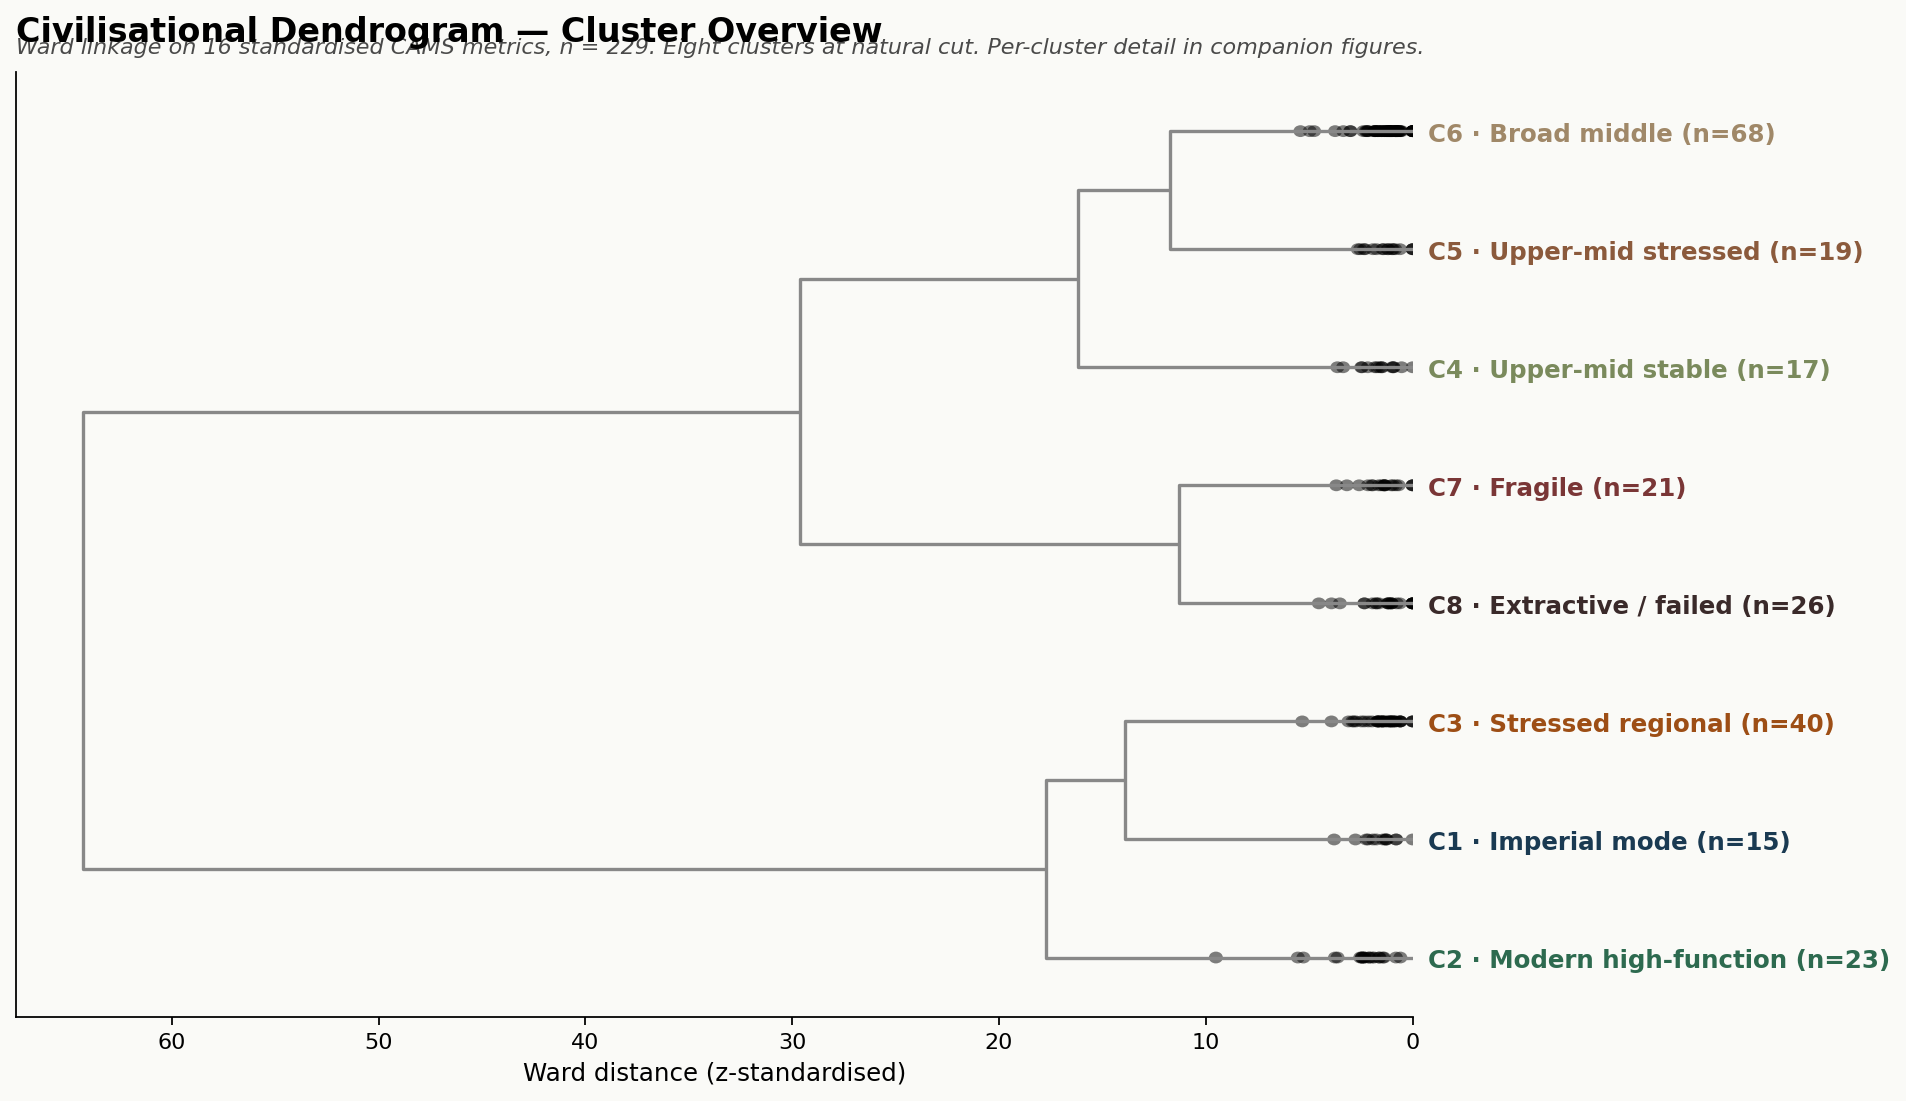
\includegraphics[width=\textwidth]{civilisations_dendrogram_overview}
  \caption{\textbf{Civilisational Dendrogram --- Cluster Overview.} Ward linkage on 16 standardised CAMS metrics, $n = 229$. Eight clusters at the natural cut. Per-cluster internal structure in Appendix~A.}
  \label{fig:dendrogram}
\end{figure}

\begin{figure}[p]
  \centering
  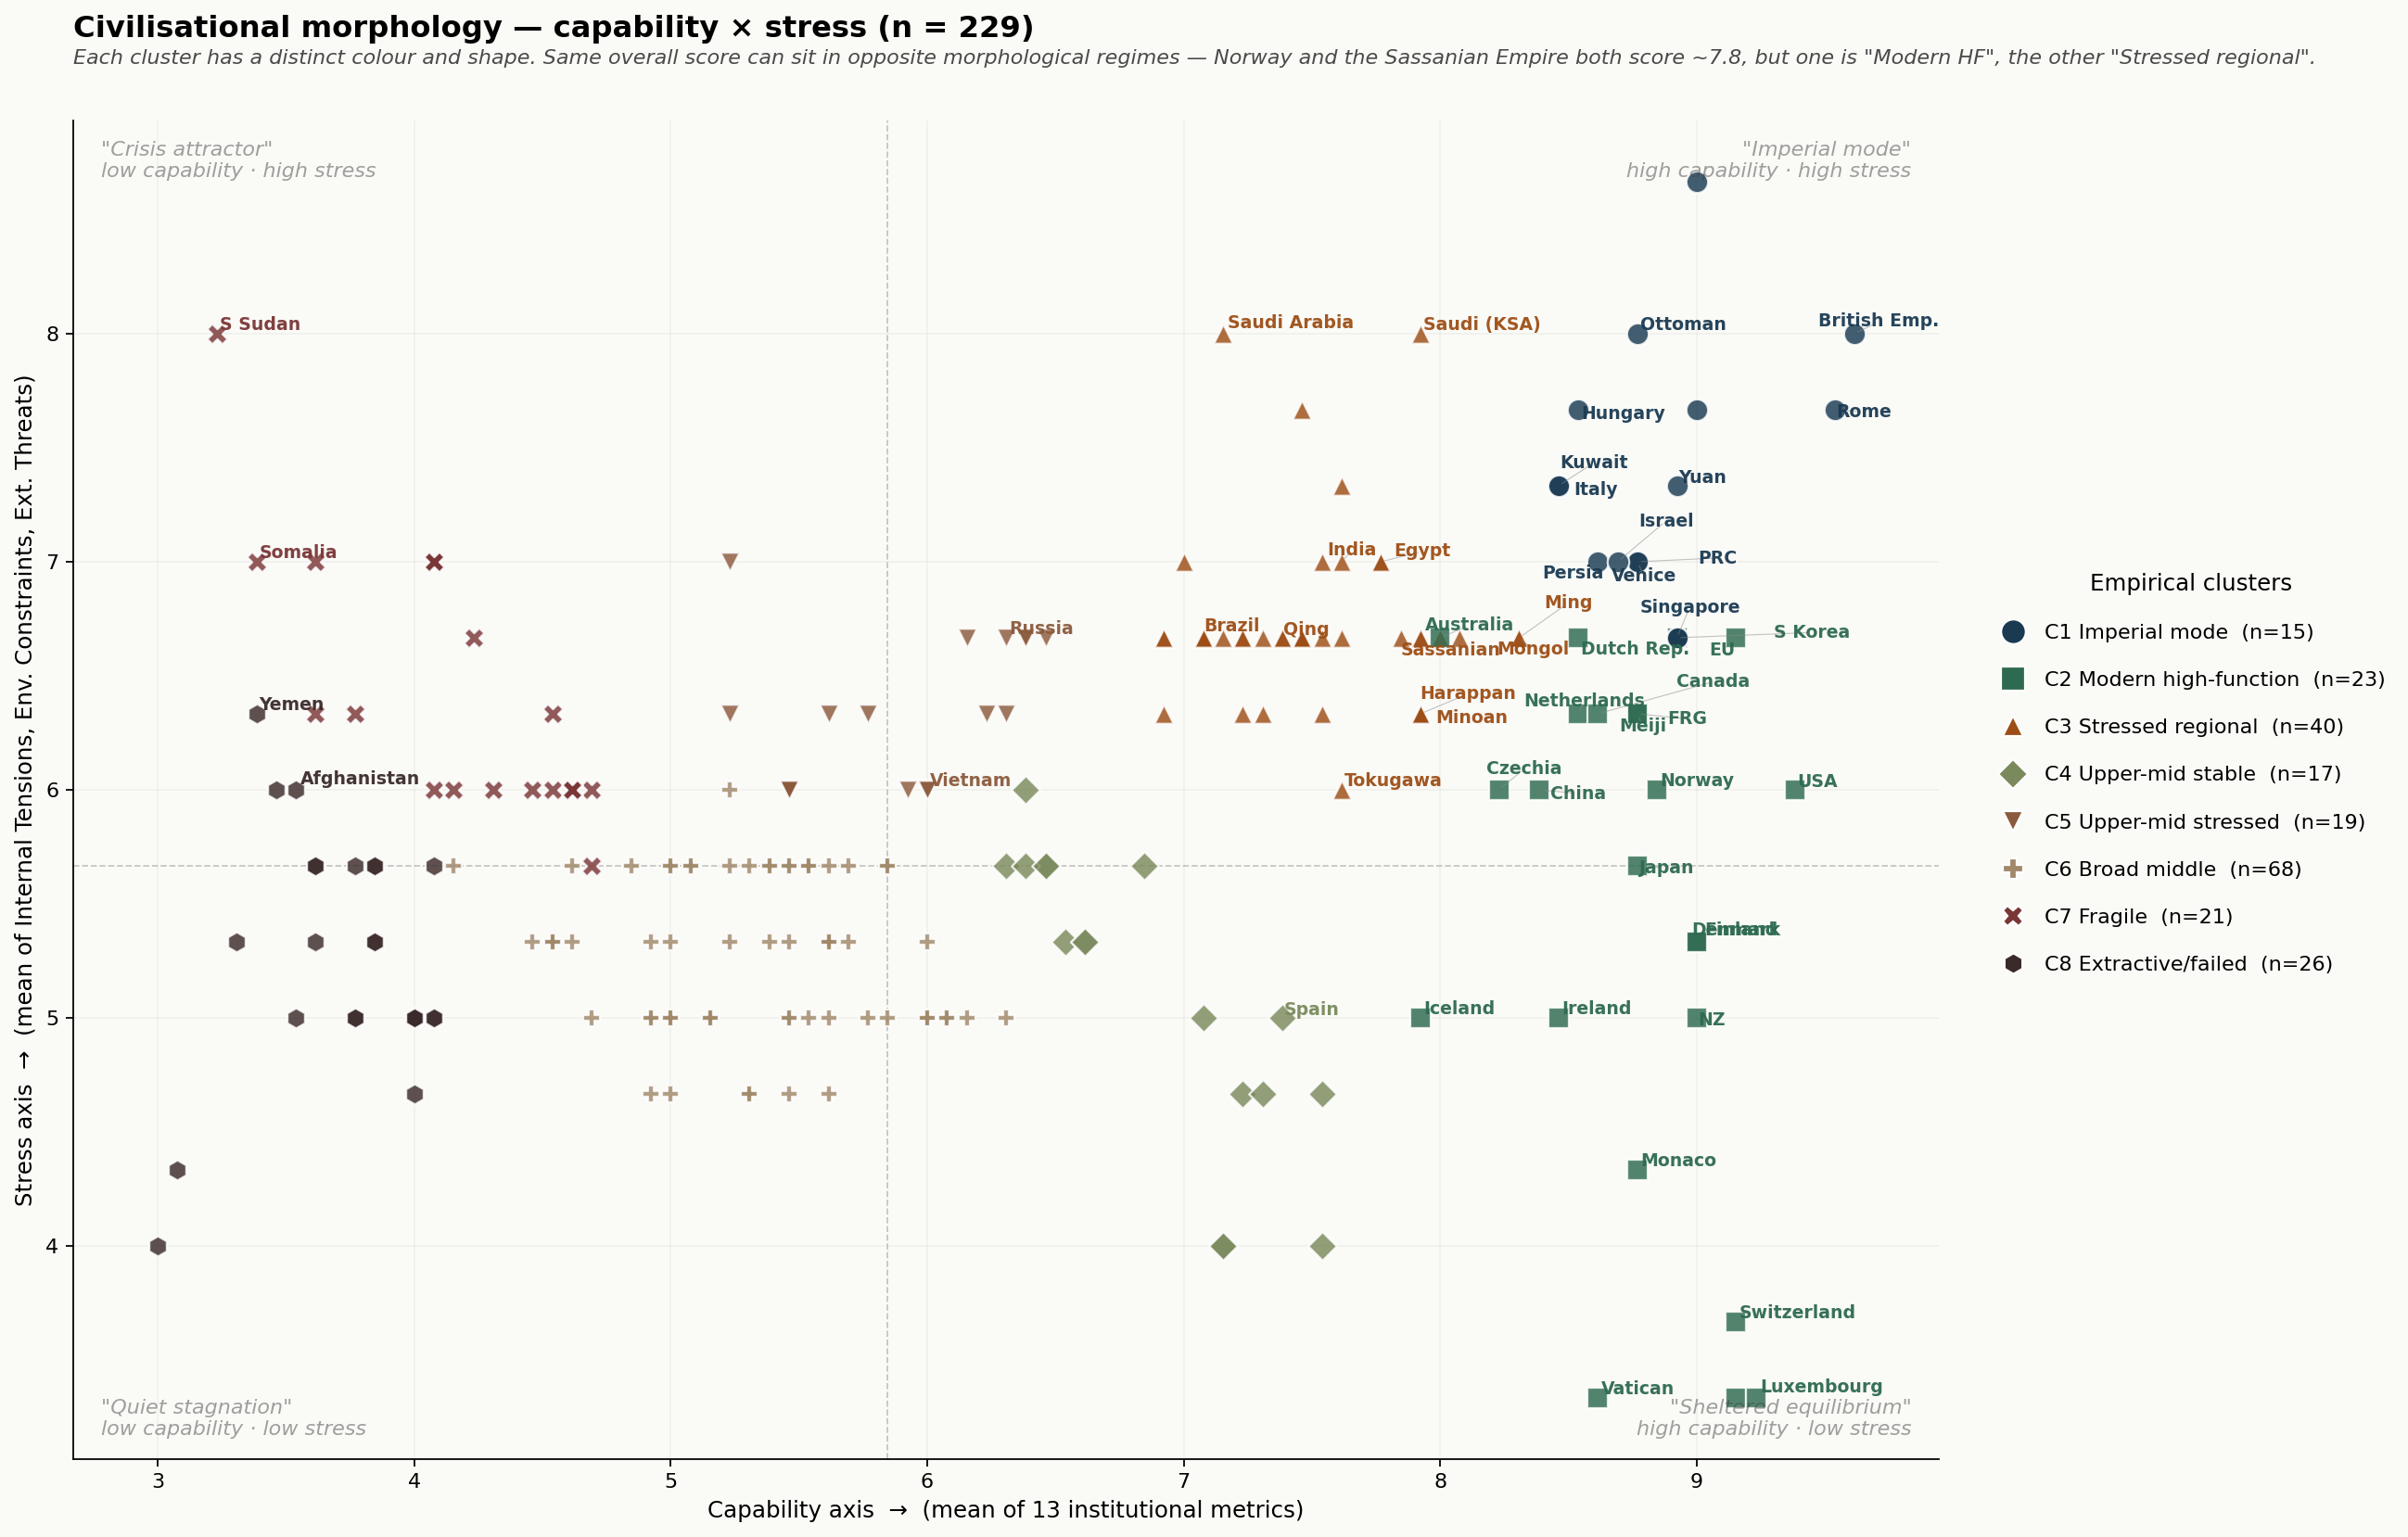
\includegraphics[width=\textwidth]{civilisations_morphology}
  \caption{\textbf{Civilisational morphology --- capability~$\times$~stress ($n = 229$).} Each cluster has a distinct colour and shape. The same overall score can sit in opposite morphological regimes: Norway and the Sassanian Empire both score $\approx 7.8$, but one is ``Modern HF'', the other ``Stressed regional''.}
  \label{fig:morphology}
\end{figure}

\subsection{The Eight Clusters}

\begin{table}[ht]
\centering
\setlength{\tabcolsep}{8pt}
\renewcommand{\arraystretch}{1.25}
\begin{tabularx}{\textwidth}{l l r r r X}
\toprule
\rowcolor{tablehead}
\textbf{Cluster} & \textbf{Label} & \textbf{$n$} & \textbf{Score} & \textbf{Stress} & \textbf{Character} \\
\midrule
C1 & Imperial mode          & 15 & 8.59 & 7.40 & High capability under sustained high stress \\
C2 & Modern high-function   & 23 & 8.13 & 5.45 & High capability under moderate stress \\
C3 & Stressed regional      & 40 & 7.38 & 6.74 & High-moderate capability under sustained pressure \\
C4 & Upper-mid stable       & 17 & 6.54 & 5.08 & Established middle tier, moderate-stress conditions \\
C5 & Upper-mid stressed     & 19 & 5.94 & 6.32 & Middle tier under elevated pressure \\
C6 & Broad middle           & 68 & 5.33 & 5.27 & Functional but constrained --- the modal world \\
C7 & Fragile                & 21 & 4.60 & 6.40 & Eroding capacity under elevated pressure \\
C8 & Extractive / failed    & 26 & 4.02 & 5.26 & Coordination collapse \\
\bottomrule
\end{tabularx}
\caption{The eight empirical clusters derived from Ward's hierarchical clustering on $z$-standardised CAMS metrics across 229 polities (mean overall score and mean stress score shown).}
\label{tab:clusters}
\end{table}

\subsection{Mapping Clusters to Coordination Morphologies}

\textbf{Cluster C1 --- Imperial mode} contains polities that have solved all eight coordination problems at large scale under sustained stress. Members include Rome, the British Empire, France, Germany, the Ottoman Empire, the Yuan Dynasty, the Republic of Venice, the People's Republic of China, the State of Israel, Hungary, Persia (Achaemenid), Italy, Singapore, and Kuwait. The cluster contains riverine-bureaucratic exemplars (PRC, Persia), maritime-trade exemplars (British Empire, Venice, Singapore), and continental exemplars (France, Germany, Ottoman, Yuan). What unites them is the capability/stress signature, not the morphological type.

\textbf{Cluster C2 --- Modern high-function} contains polities operating capable institutions under moderate stress. Members include the United States, the European Union, South Korea, Finland, Meiji Japan, Norway, Denmark, the Federal Republic of Germany, New Zealand, Japan, the Dutch Republic, Canada, Luxembourg, Netherlands, Switzerland, Liechtenstein, Monaco, Ireland, the Czech Republic, Australia, Vatican City, Iceland, and historical China. This cluster is dominated by maritime-modular and insular morphologies but also includes continental polities under modern-democratic configurations.

\textbf{Cluster C3 --- Stressed regional} is the largest high-tier cluster ($n = 40$) and contains the structural majority of historically capable polities. Members include the riverine-bureaucratic empires (Ming, Qing, Jin, Egypt, Sassanian Persia, Harappan), the steppe and Eurasian empires (Mongol, Parthian, Khitan Liao, Sogdian, Timurid, Tibetan), the Mediterranean trade republics that did not reach apex capability (Phoenician, Etruscan, Minoan, Mycenaean), South and Southeast Asian composite polities (India, Vietnam, Thailand, Indonesia, Philippines, Brazil, Botswana, South Africa), and the contemporary Middle Eastern major polities (Iran, Saudi Arabia, Turkey). The morphological diversity within C3 is the strongest evidence that morphology and capability/stress level are partially independent.

\textbf{Clusters C4--C5} distinguish established middle-tier polities from those under elevated stress. C4 contains stable post-industrial democracies of the European periphery and Latin American emerging economies; C5 contains stressed continental polities including Russia, post-Soviet states, and several Middle Eastern and Central Asian polities under sustained pressure.

\textbf{Clusters C7--C8} distinguish fragile from collapsed coordination. The boundary between them is gated by stress signature rather than capability level: C7 and C8 have similar capability levels (4.6 vs.\ 4.0) but C7 carries higher stress (6.4 vs.\ 5.3). C7 polities are at greatest dynamic risk of cascading into C8.

\subsection{The Apex Split}

The most consequential structural finding is that what appears in raw scoring as a single apex tier of high-capability polities resolves under clustering into two genuinely distinct ecological regimes---Imperial mode (C1) and Modern high-function (C2). They have nearly identical capability scores but differ sharply on stress signature. This is not a difference of regime type or development stage. It is a difference of \textit{which coordination problems are currently dominant}: Imperial-mode polities are managing high-amplitude stress as their primary operational challenge; Modern-high-function polities are managing legitimacy renewal and integration as theirs.

Imperial-mode polities are stress-processing systems first; their characteristic failure mode is \textit{Type~I phantom collapse}---sustained high abstraction~$\times$~coherence ($A \cdot C$) persisting while material capacity drains underneath, with Rome's 200--450~CE trajectory as the historical paradigm~\cite{mckern2026esch,mckern2026v32r}.

\subsection{Geographic Recovery}

The cluster algorithm does not separate riverine from maritime morphologies into different clusters because their static institutional metrics overlap; both can sit in C1 or C3 depending on capability and stress level. The morphological distinction lives in the \textit{pattern of node weightings within the cluster} rather than in cluster membership. This is a scope condition for the taxonomy: static-metric clustering identifies coordination \textit{regimes} (capability~$\times$~stress configurations); within-cluster analysis of node weightings identifies coordination \textit{morphologies} (which nodes carry the architecture). Both analytical levels are required for a complete reading of the data.

% ─────────────────────────────────────────────────────────────────────────────
\section{Placements That Resist Conventional Framings}
% ─────────────────────────────────────────────────────────────────────────────

Three placements warrant explicit comment because they cut against routine Western framings of contemporary geopolitics.

The \textbf{People's Republic of China} clusters with Imperial mode---that is, with Rome, the British Empire, the Ottoman Empire, France, Germany, Yuan, Persia, and Venice. This is a structural finding, not an ideological one. It places the PRC within the empire-shaped coordination lineage that includes the Western polities themselves. Framings of the PRC as a categorically other or uniquely opaque type of system do not survive structural inspection. The PRC is operating in the same ecological regime that European empires operated in during their high-capability phases, with similar institutional architecture and similar dynamic risks.

The \textbf{United States} clusters with Modern high-function---that is, with Japan, South Korea, the Federal Republic of Germany, the EU, Canada, Australia, and the Nordics. Its capability score is the highest in the corpus (9.4) but its stress signature (6.0) is moderate by C1 standards. American foreign-policy rhetoric routinely implies imperial-mode operation, but the structural signature is closer to Japan and Germany than to Rome and Britain. Whether this represents structural evolution beyond imperial mode, or simply that the relevant internal stresses have not yet pushed the signature into C1, is an open dynamical question.

The \textbf{Russian Federation} clusters in C5 (Upper-mid stressed), with capability around 6.3 and stress around 6.7. This places it structurally alongside Mexico, Croatia, Bahrain, Cyprus, and Jordan. It is neither a uniquely threatening actor nor a uniquely capable one. It is a stressed upper-middle polity processing the Ukraine war, comprehensive sanctions, the ageing of its administrative infrastructure, and unresolved transition from the Soviet period. The data support this reading without recourse to either Russophobic or revanchist framings.

These placements are not normative claims. They are what falls out of standard hierarchical clustering applied to the standardised metrics. Their value to the taxonomic project is precisely that they resist the dominant rhetorical framings while remaining defensible from the data. A taxonomy that recovered conventional Western political categories would be of less analytical value than one that recovers structural similarities cutting across them.

% ─────────────────────────────────────────────────────────────────────────────
\section{Falsifiability of the Taxonomic Claim}
% ─────────────────────────────────────────────────────────────────────────────

A taxonomy without falsifiability conditions is description, not science. The following criteria define the next stage of empirical testing for the taxonomic claim specifically.

\begin{enumerate}[leftmargin=1.8em, label=\textbf{\arabic*.}]

\item \textbf{Cluster Stability Test.} Independent researchers, applying the published scoring protocol to the same corpus, should recover clusters with substantial agreement (adjusted Rand index $\geq 0.65$). Lower agreement indicates that clustering depends substantially on idiosyncratic scoring choices.

\item \textbf{Out-of-Sample Cluster Assignment Test.} Polities not used in the framework's development---including pre-modern non-Eurasian polities, contemporary firms scored against the same protocol, and contemporary subnational entities---should be assignable to the eight clusters without requiring the introduction of new clusters.

\item \textbf{Cross-Method Recovery Test.} Alternative clustering methods ($k$-means with silhouette optimisation, DBSCAN, average-linkage hierarchical clustering, community detection on a similarity network) applied to the same standardised metrics should recover qualitatively similar groupings.

\item \textbf{Apex-Split Robustness Test.} The C1/C2 split should survive (a) removal of any single distinguishing metric, (b) decoupled scoring of the stress dimensions from independent evidence streams, and (c) variation in standardisation method.

\item \textbf{Coordination-Problem Recovery Test.} If the eight nodes correspond to genuine recurring coordination problems, then within-cluster variation should be interpretable as differential weighting on the eight problems rather than as random noise. Pre-registered predictions about which morphologies will weight which nodes (riverine $\rightarrow$ Stewards + Archive; maritime $\rightarrow$ Flow + Helm; continental $\rightarrow$ Shield + Helm) should be empirically recoverable from cluster sub-structure.

\item \textbf{Geographic Sub-Structure Test.} Morphological types should be recoverable as sub-structure within the larger clusters (especially C3) without geographic labels supplied to the recovery procedure.

\item \textbf{Trajectory Coherence Test.} Time-series analysis of polities at cluster boundaries should show coherent trajectories rather than random fluctuation. A polity moving from C2 into C1, for example, should display rising stress signature with capability roughly preserved.

\end{enumerate}

These criteria are deliberately demanding. The taxonomy should fail at least some of them if it is mistaken in any non-trivial respect.

% ─────────────────────────────────────────────────────────────────────────────
\section{Conclusion}
% ─────────────────────────────────────────────────────────────────────────────

The eight clusters this paper presents are not a ranking. They are morphologies---configurations of the same underlying coordination grammar, differentiated by capability level, stress regime, and the relative weighting of slow-loop and fast-loop nodes that geography and history have produced.

The argument has run from the bottom up. Eight recurring coordination problems are imposed on Holocene human societies by ecology and scale. Geography makes some of these problems acute and others latent in any given environment, selecting for differential institutional weightings. Local solutions accumulate, through capacity formation, bond-strength accretion, and solution-by-extension, into morphologically locked-in architectures whose persistence outlasts the political regimes that operate them. The eight-node CAMS grammar is the minimal functional decomposition at which these architectures become surveyable; it maps one node to each recurring problem; its warrant is empirical, lying in the structure that hierarchical clustering recovers without geographic priors. The eight clusters that emerge---Imperial, Modern High-Function, Stressed Regional, Upper-Mid Stable, Upper-Mid Stressed, Broad Middle, Fragile, Extractive---are the empirical record of how human societies have actually configured themselves.

The implication for \textit{common global interests} is that, despite morphological differences, all polities share the same physical envelope. The eight coordination problems are imposed, in the end, by the same physics: energy throughput is finite, entropy production is unavoidable, information has acquisition costs, climate forcing is system-wide. These constraints do not respect coordination morphology. The morphological diversity the taxonomy reveals is the human species' adaptive repertoire under shared constraints, not a contest between rival civilisational projects with winners and losers. The common interest lies in maintaining the global niche-construction substrate that supports any high-coordination polity at all.

Two questions remain open and require companion treatment. The formal mechanism of path dependency itself---what determines when a morphology is preserved against shocks and when it can be deliberately changed---is developed in the companion paper on the Library Attractor~\cite{mckern2026library}. The cliodynamic and EES integration of the taxonomy is the subject of continuing elaboration.

The framework will, on its own terms, be wrong if it cannot survive the seven falsification tests in Section~8. The datasets, scoring protocols, dendrograms, and reproducible code are publicly available at \href{https://neuralnations.org}{neuralnations.org} and \href{https://github.com/KaliBond/wintermute}{github.com/KaliBond/wintermute}. Researchers are invited to replicate, extend, and challenge these results.

% ─────────────────────────────────────────────────────────────────────────────
%  REFERENCES
% ─────────────────────────────────────────────────────────────────────────────
\newpage
\begin{thebibliography}{99}

\bibitem{prigogine1984}
Prigogine, I. \& Stengers, I. (1984). \textit{Order Out of Chaos: Man's New Dialogue with Nature}. Bantam Books.

\bibitem{laland2015}
Laland, K.\,N., Uller, T., Feldman, M.\,W., Sterelny, K., M\"{u}ller, G.\,B., Moczek, A., Jablonka, E. \& Odling-Smee, J. (2015). The extended evolutionary synthesis: its structure, assumptions and predictions. \textit{Proceedings of the Royal Society B}, 282(1813), 20151019.

\bibitem{tainter1988}
Tainter, J.\,A. (1988). \textit{The Collapse of Complex Societies}. Cambridge University Press.

\bibitem{boyd1985}
Boyd, R. \& Richerson, P.\,J. (1985). \textit{Culture and the Evolutionary Process}. University of Chicago Press.

\bibitem{odlingsmee2003}
Odling-Smee, F.\,J., Laland, K.\,N. \& Feldman, M.\,W. (2003). \textit{Niche Construction: The Neglected Process in Evolution}. Princeton University Press.

\bibitem{turchin2003}
Turchin, P. (2003). \textit{Historical Dynamics: Why States Rise and Fall}. Princeton University Press.

\bibitem{mckern2026paper1}
McKern, K.\,F. (2026). Paper 1: The Complex Adaptive Meta-System. \textit{NeuralNations Working Papers}.

\bibitem{mckern2026paper2}
McKern, K.\,F. (2026). Paper 2: A Natural Taxonomy of Meta-Systems. \textit{NeuralNations Working Papers}.

\bibitem{mckern2026esch}
McKern, K.\,F. (2026). CAMS Extended Social Cognition Hypothesis (ESCH). \textit{NeuralNations Technical Notes}.
McKern, K.\,F. (2026). CAMS Extended Social Cognition Hypothesis (ESCH). \textit{NeuralNations Technical Notes}.

\bibitem{mckern2026v32r}
McKern, K.\,F. (2026). CAMS v3.2-R: Retrospective Validation and Criticality Recalibration. \textit{NeuralNations Technical Notes}.

\bibitem{mckern2026usa}
McKern, K.\,F. (2026). CAMNATIONS5 USA 1996--2026 Pipeline Validation. \textit{NeuralNations Technical Notes}.

\bibitem{mckern2026library}
McKern, K.\,F. (2026). The Library Attractor: A Formal Operator of Civilisational Path Dependency. \textit{NeuralNations Technical Notes}.

\bibitem{pierson2000}
Pierson, P. (2000). Increasing returns, path dependence, and the study of politics. \textit{American Political Science Review}, 94(2), 251--267.

\end{thebibliography}

% ─────────────────────────────────────────────────────────────────────────────
%  APPENDIX — Per-Cluster Internal Dendrograms
% ─────────────────────────────────────────────────────────────────────────────
\newpage
\appendix
\section{Per-Cluster Internal Dendrograms}
\label{app:dendrograms}

The following figures show the internal Ward-linkage structure within each of the eight empirical clusters. Ward distance is $z$-standardised within each cluster.

\begin{figure}[p]
  \centering
  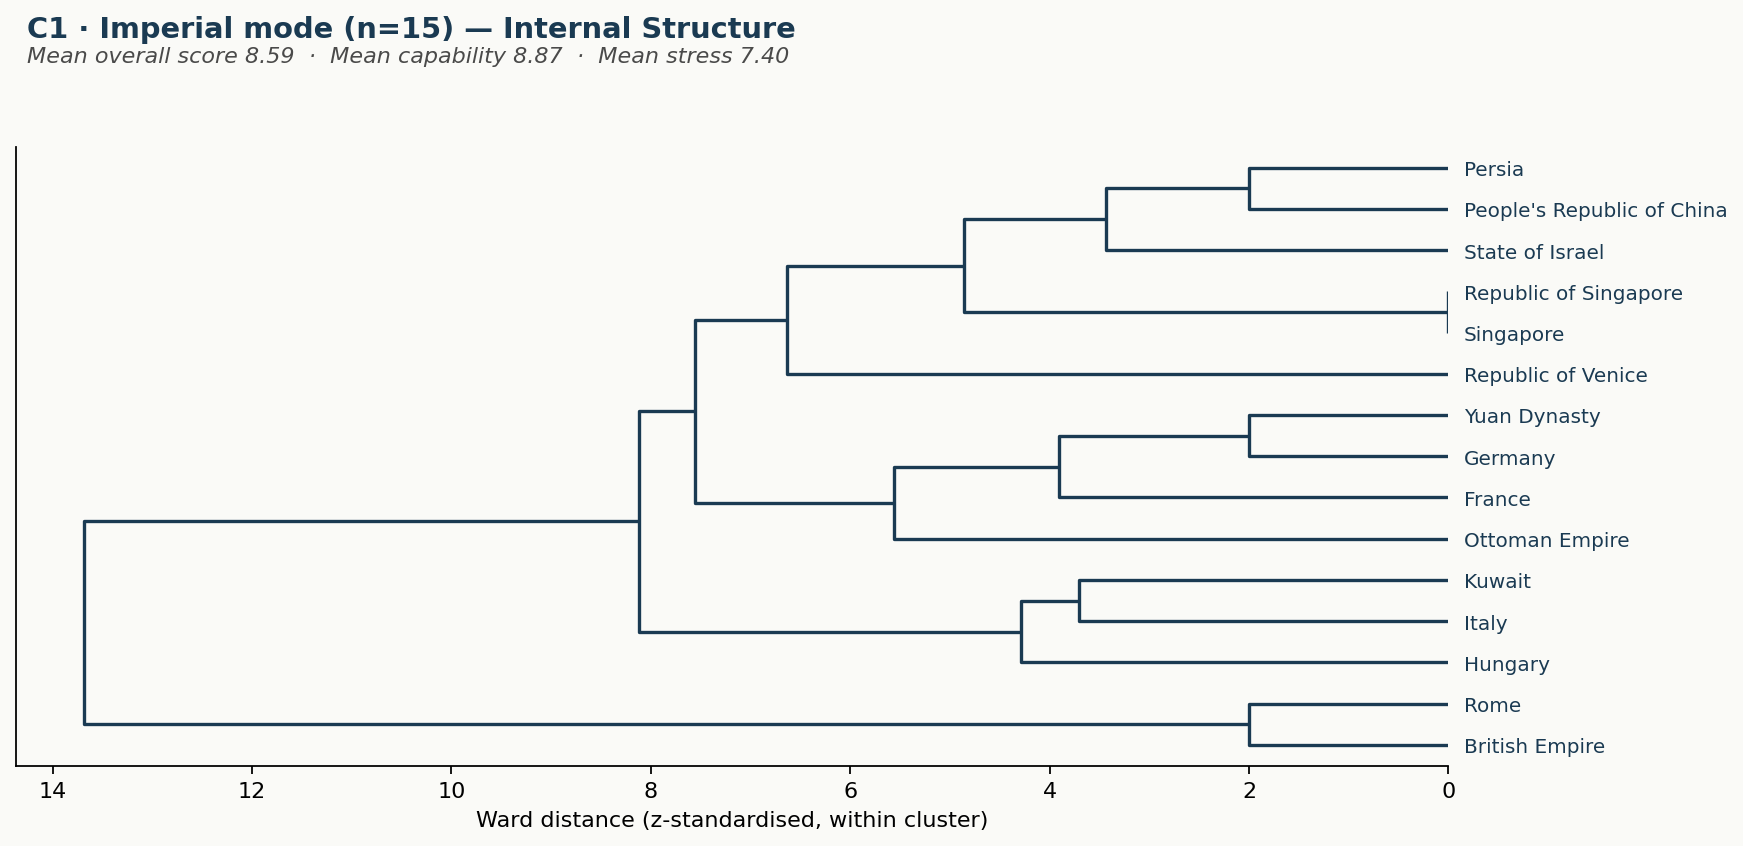
\includegraphics[width=\textwidth, height=0.82\textheight, keepaspectratio]{dendro_C1_Imperial_mode}
  \caption{\textbf{C1 $\cdot$ Imperial mode ($n=15$) --- Internal Structure.} Mean overall score 8.59 $\cdot$ Mean capability 8.87 $\cdot$ Mean stress 7.40.}
  \label{fig:c1}
\end{figure}

\begin{figure}[p]
  \centering
  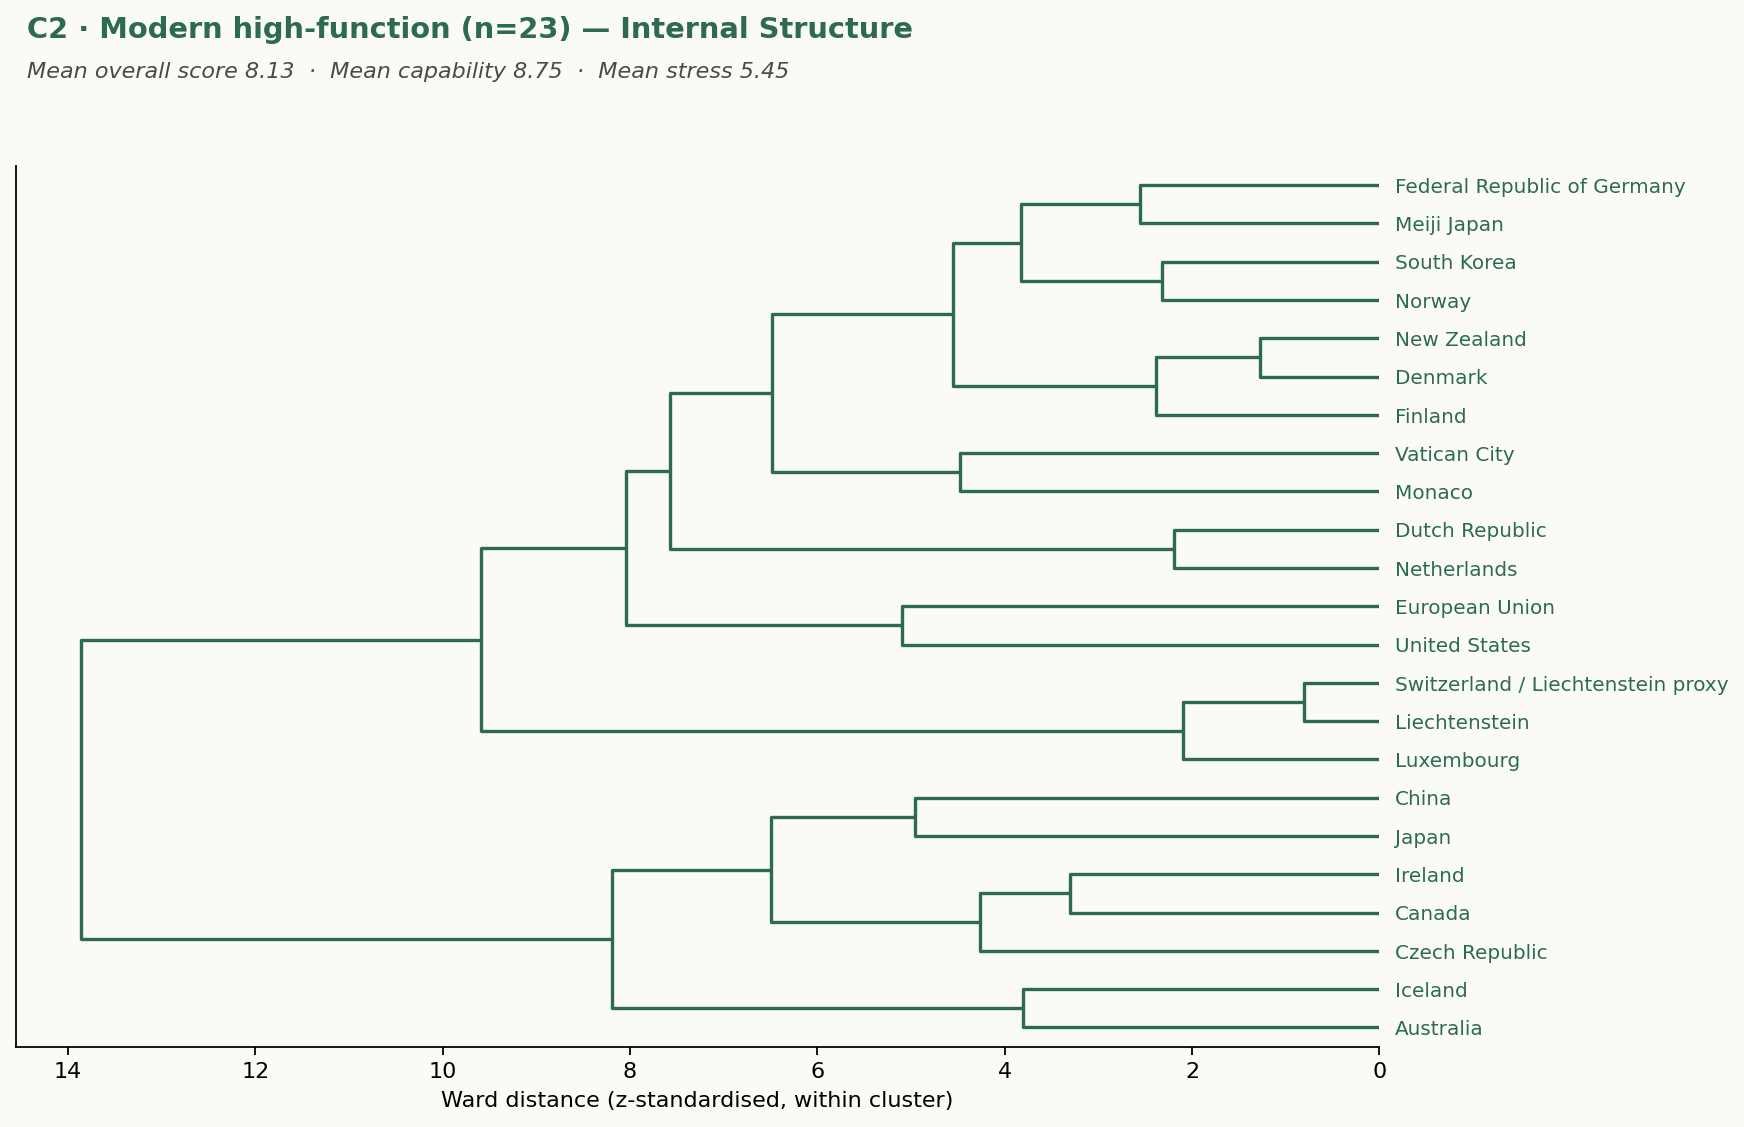
\includegraphics[width=\textwidth, height=0.82\textheight, keepaspectratio]{dendro_C2_Modern_high_function}
  \caption{\textbf{C2 $\cdot$ Modern high-function ($n=23$) --- Internal Structure.} Mean overall score 8.13 $\cdot$ Mean capability 8.75 $\cdot$ Mean stress 5.45.}
  \label{fig:c2}
\end{figure}

\begin{figure}[p]
  \centering
  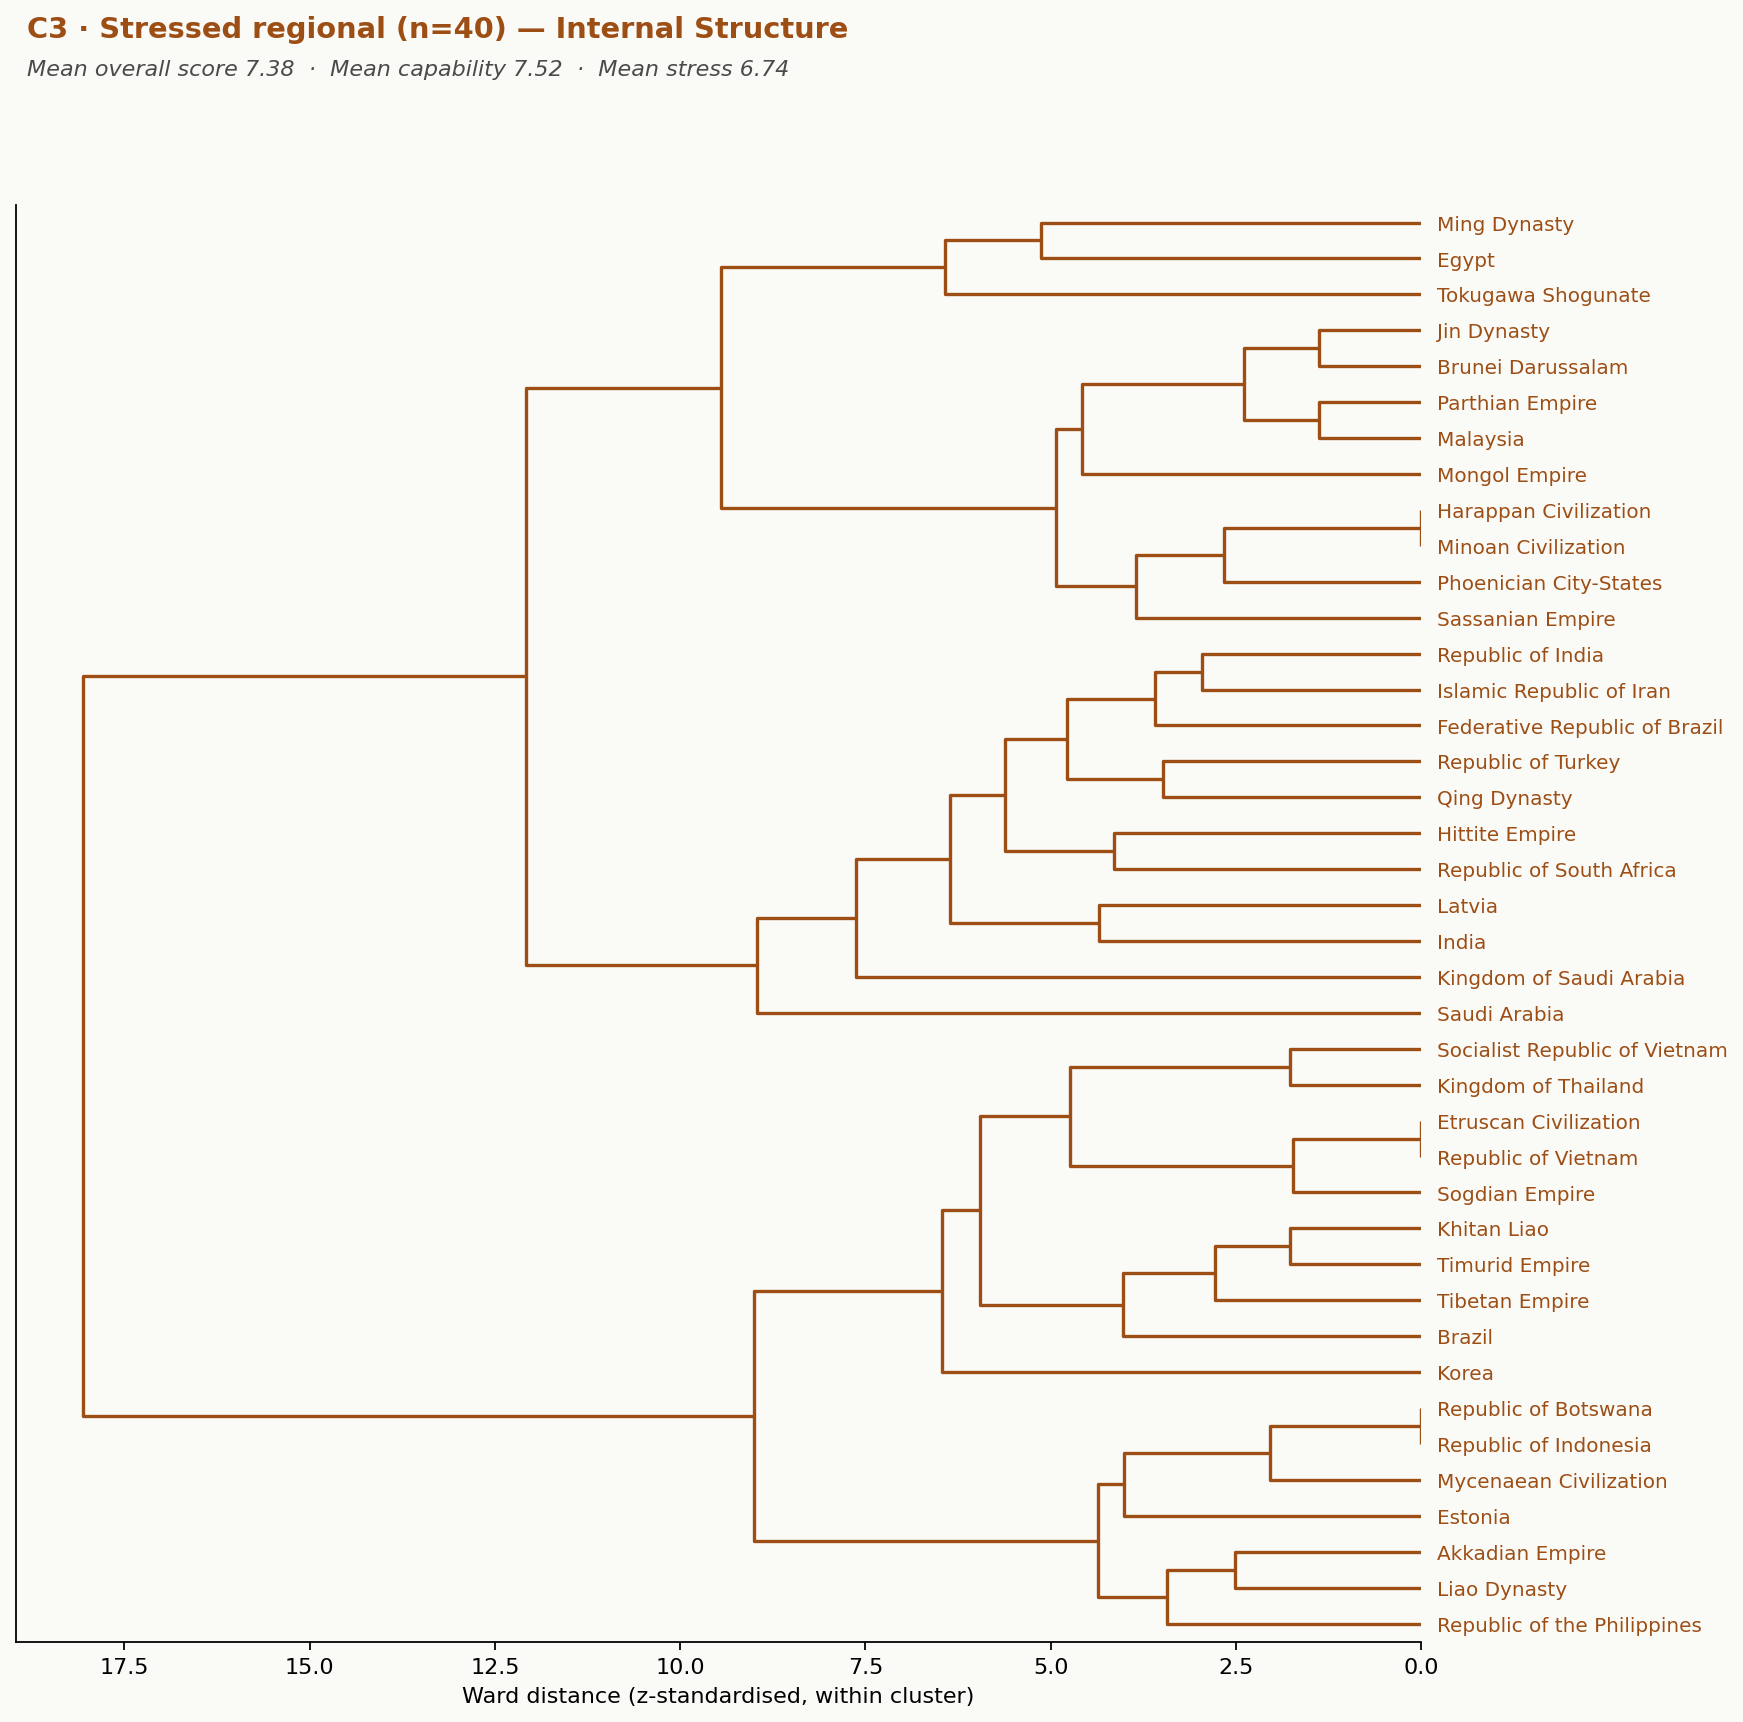
\includegraphics[width=\textwidth, height=0.82\textheight, keepaspectratio]{dendro_C3_Stressed_regional}
  \caption{\textbf{C3 $\cdot$ Stressed regional ($n=40$) --- Internal Structure.} Mean overall score 7.38 $\cdot$ Mean capability 7.52 $\cdot$ Mean stress 6.74.}
  \label{fig:c3}
\end{figure}

\begin{figure}[p]
  \centering
  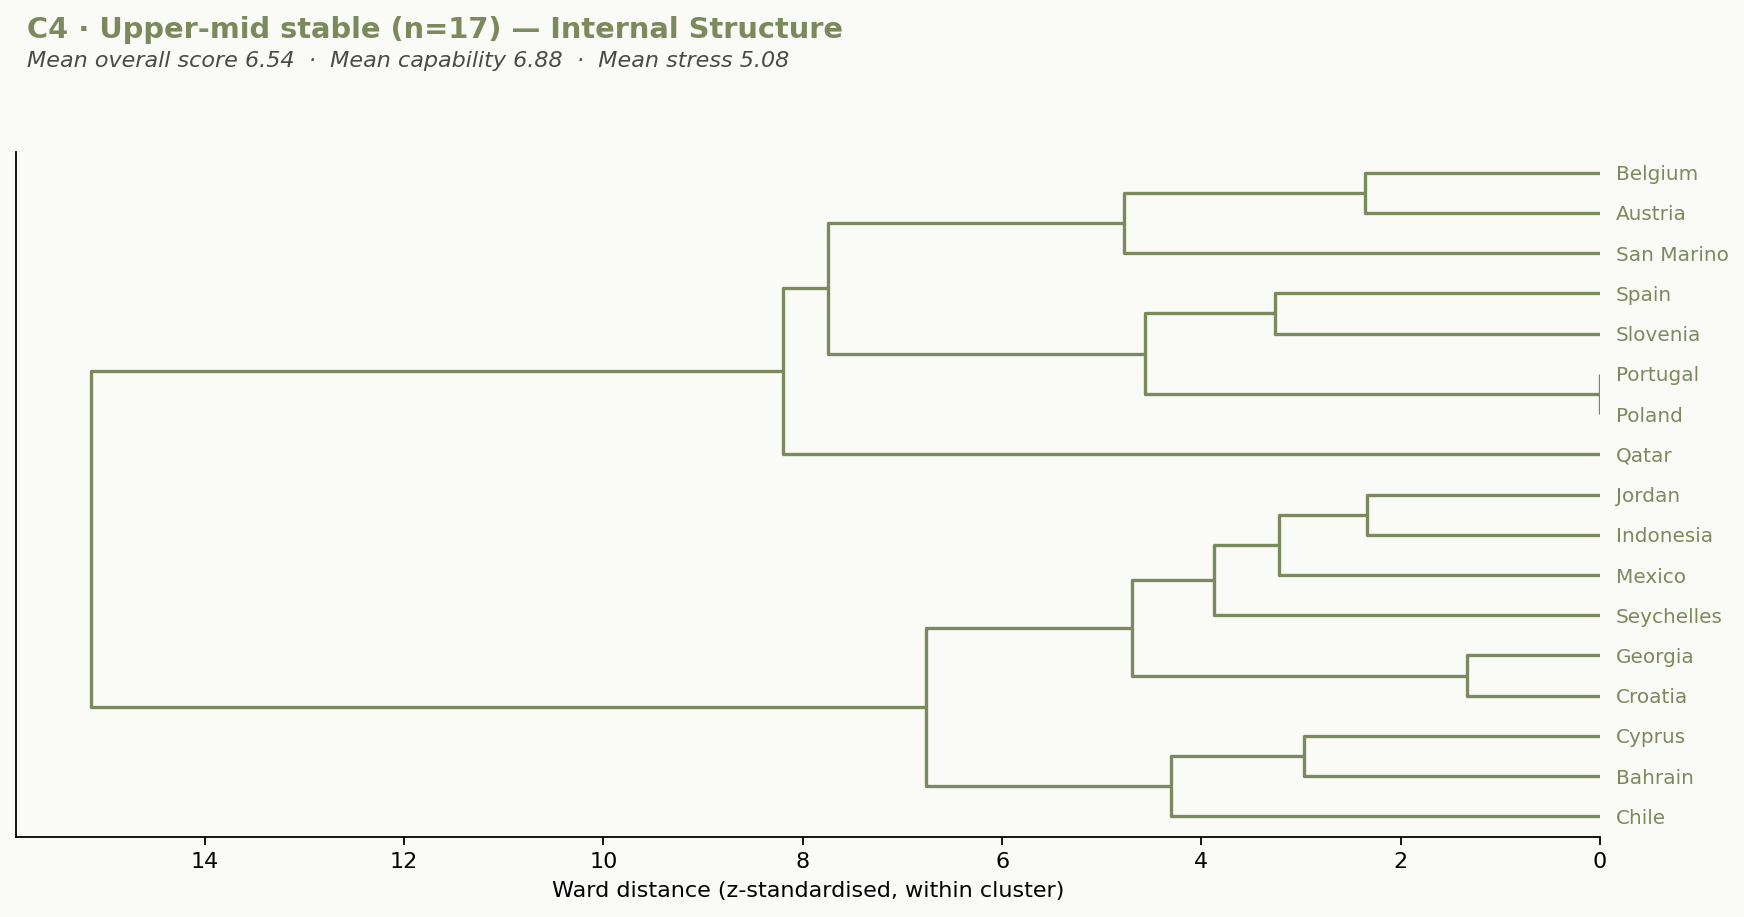
\includegraphics[width=\textwidth, height=0.82\textheight, keepaspectratio]{dendro_C4_Upper_mid_stable}
  \caption{\textbf{C4 $\cdot$ Upper-mid stable ($n=17$) --- Internal Structure.} Mean overall score 6.54 $\cdot$ Mean capability 6.88 $\cdot$ Mean stress 5.08.}
  \label{fig:c4}
\end{figure}

\begin{figure}[p]
  \centering
  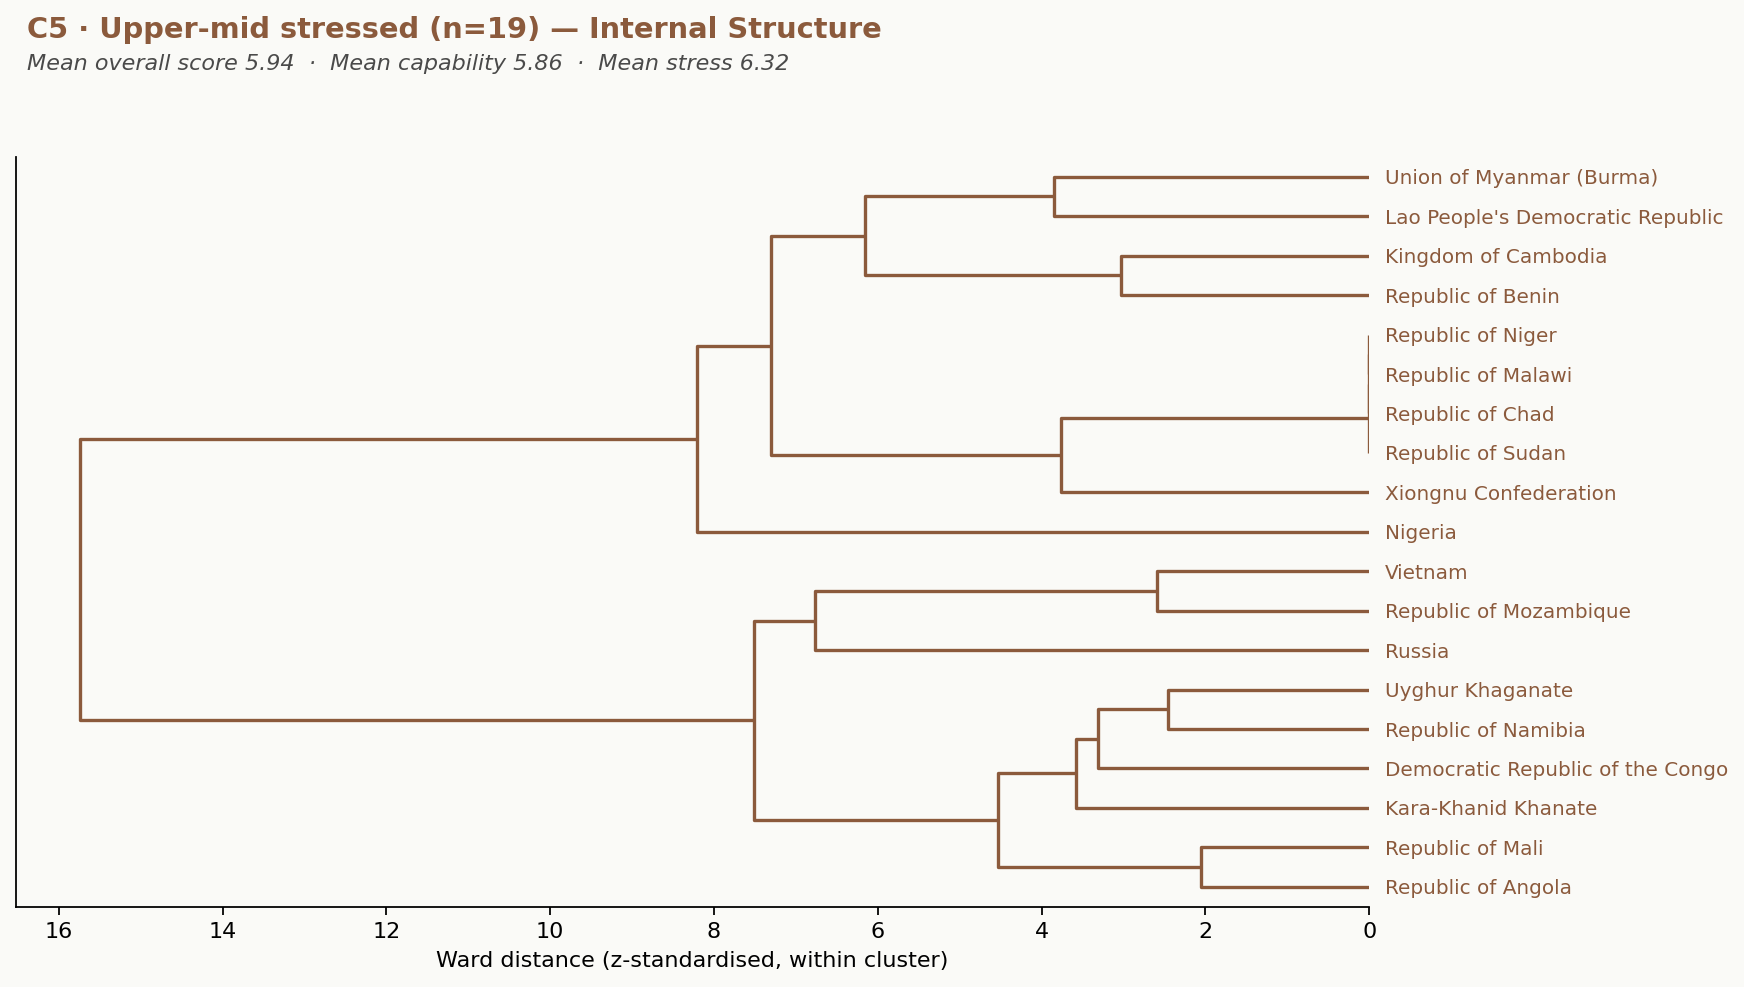
\includegraphics[width=\textwidth, height=0.82\textheight, keepaspectratio]{dendro_C5_Upper_mid_stressed}
  \caption{\textbf{C5 $\cdot$ Upper-mid stressed ($n=19$) --- Internal Structure.} Mean overall score 5.94 $\cdot$ Mean capability 5.86 $\cdot$ Mean stress 6.32.}
  \label{fig:c5}
\end{figure}

\begin{figure}[p]
  \centering
  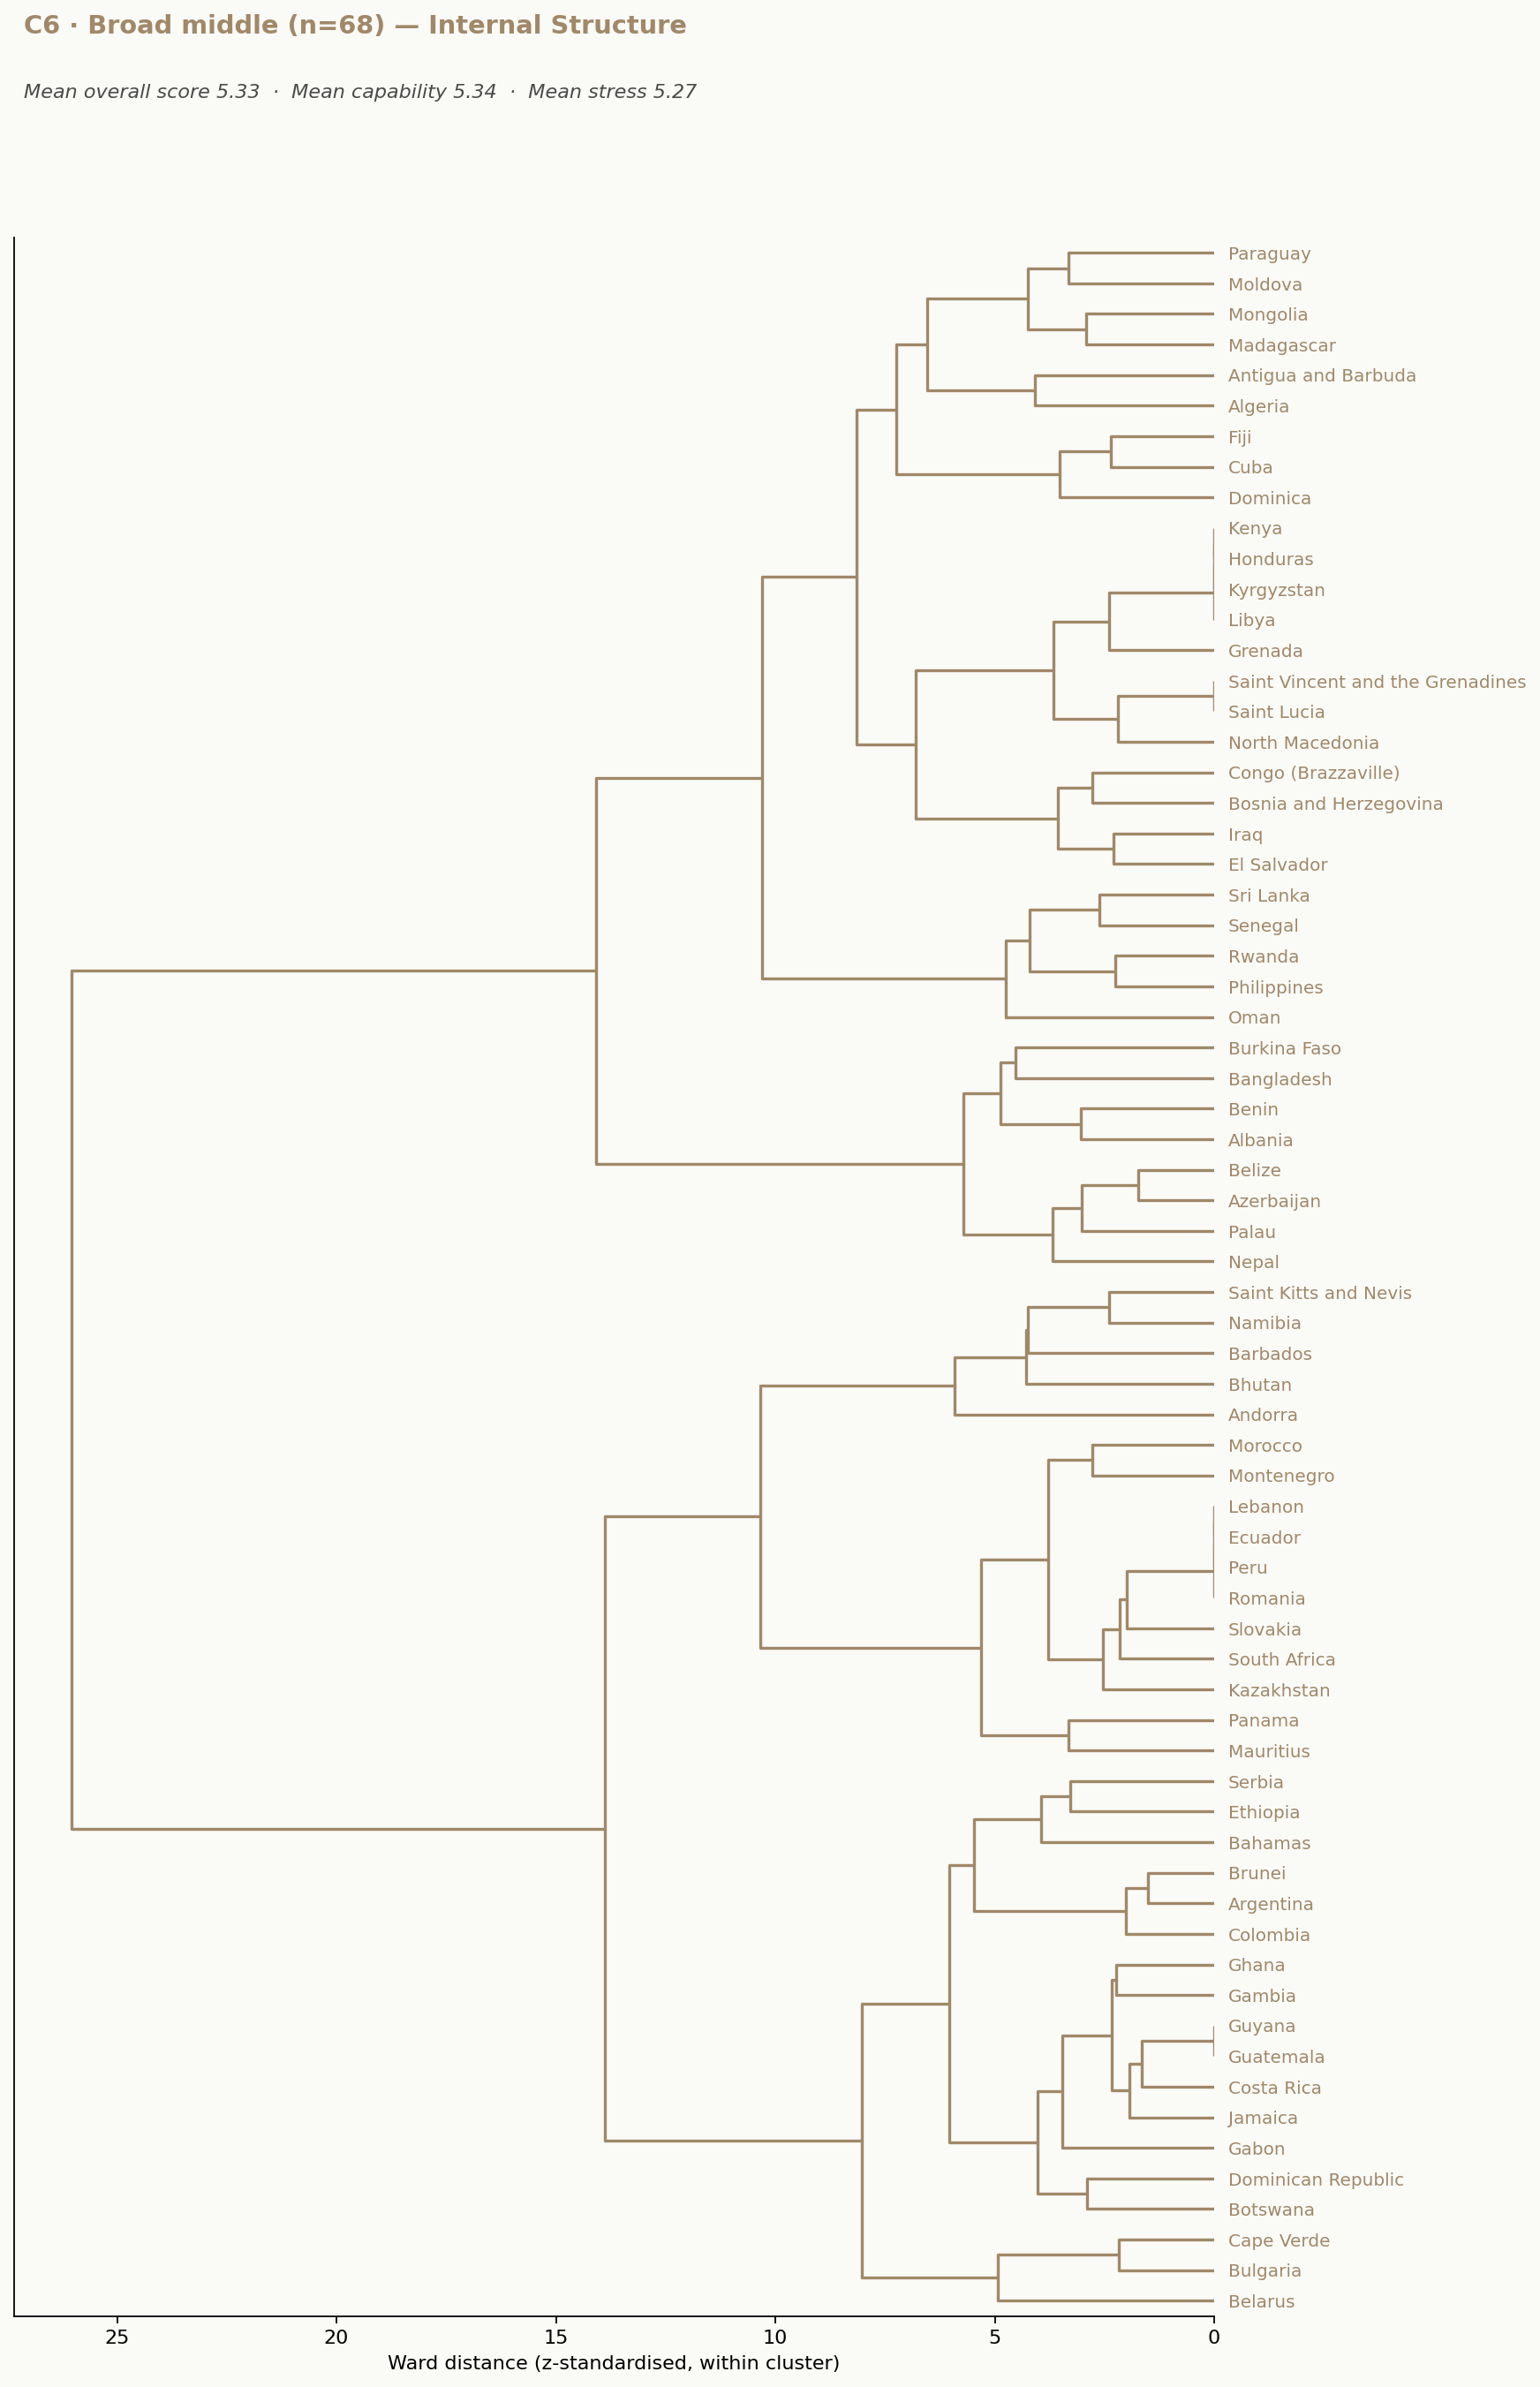
\includegraphics[width=\textwidth, height=0.82\textheight, keepaspectratio]{dendro_C6_Broad_middle}
  \caption{\textbf{C6 $\cdot$ Broad middle ($n=68$) --- Internal Structure.} Mean overall score 5.33 $\cdot$ Mean capability 5.34 $\cdot$ Mean stress 5.27.}
  \label{fig:c6}
\end{figure}

\begin{figure}[p]
  \centering
  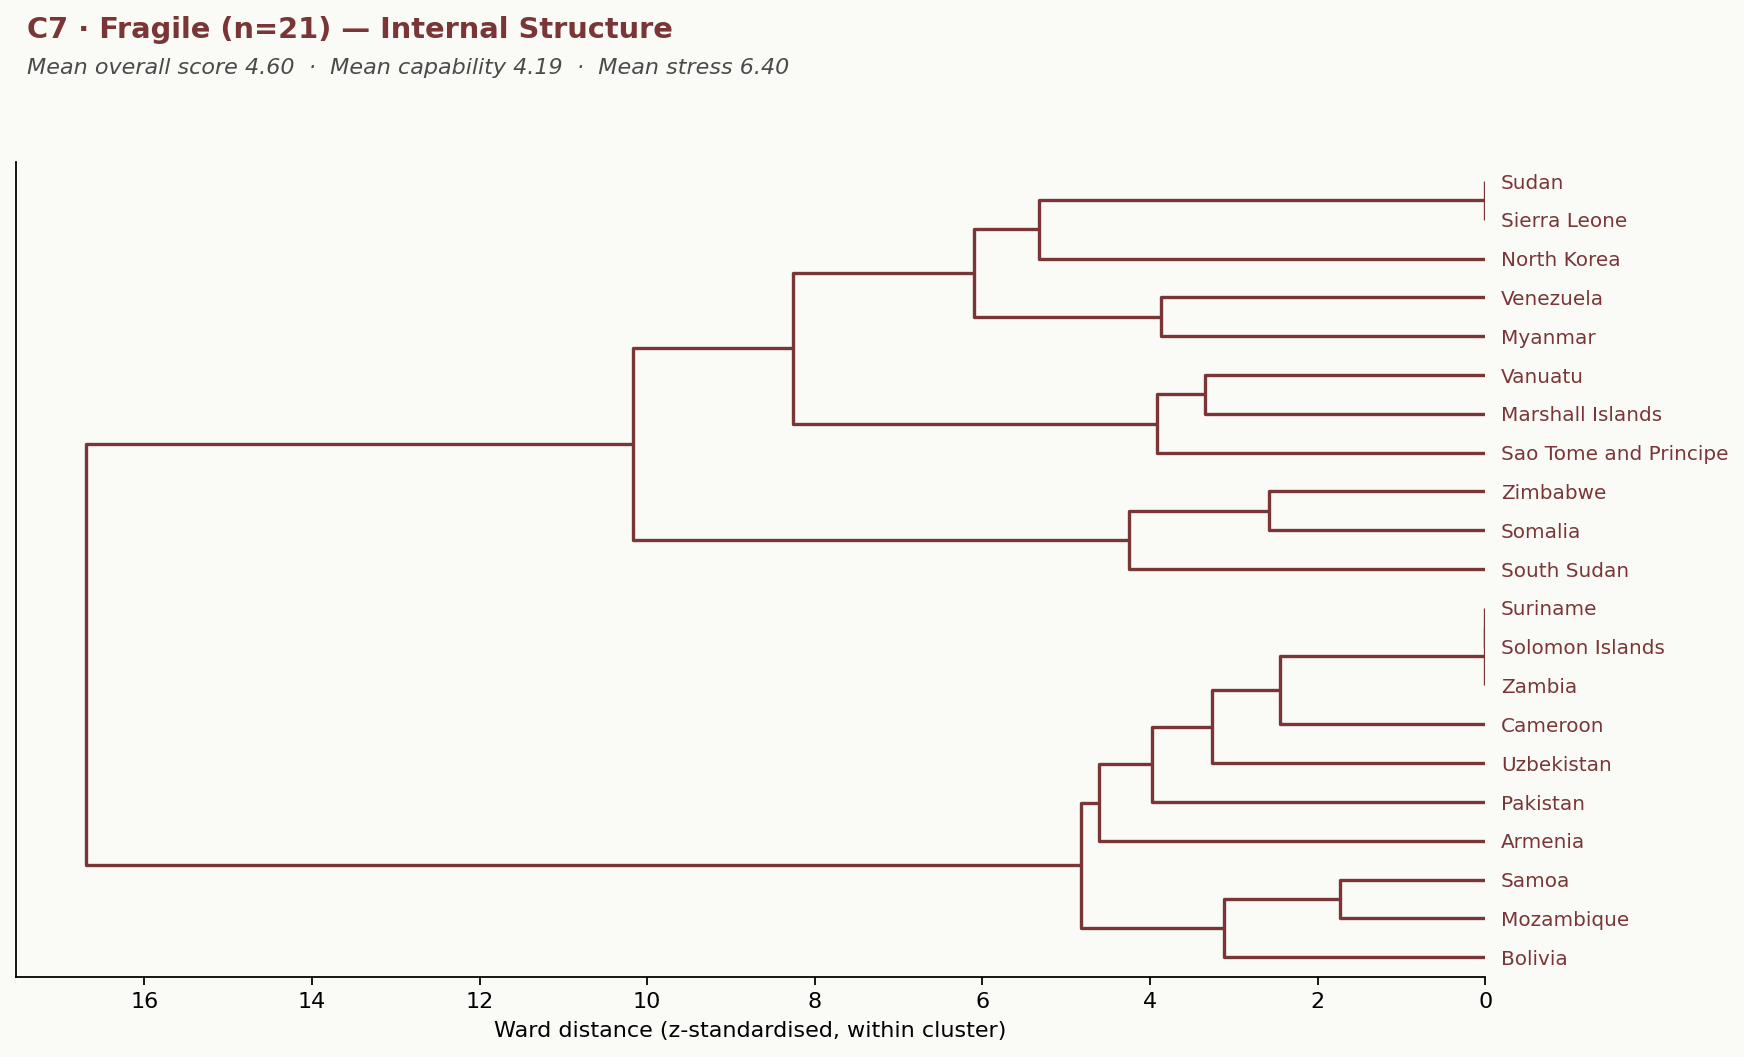
\includegraphics[width=\textwidth, height=0.82\textheight, keepaspectratio]{dendro_C7_Fragile}
  \caption{\textbf{C7 $\cdot$ Fragile ($n=21$) --- Internal Structure.} Mean overall score 4.60 $\cdot$ Mean capability 4.19 $\cdot$ Mean stress 6.40.}
  \label{fig:c7}
\end{figure}

\begin{figure}[p]
  \centering
  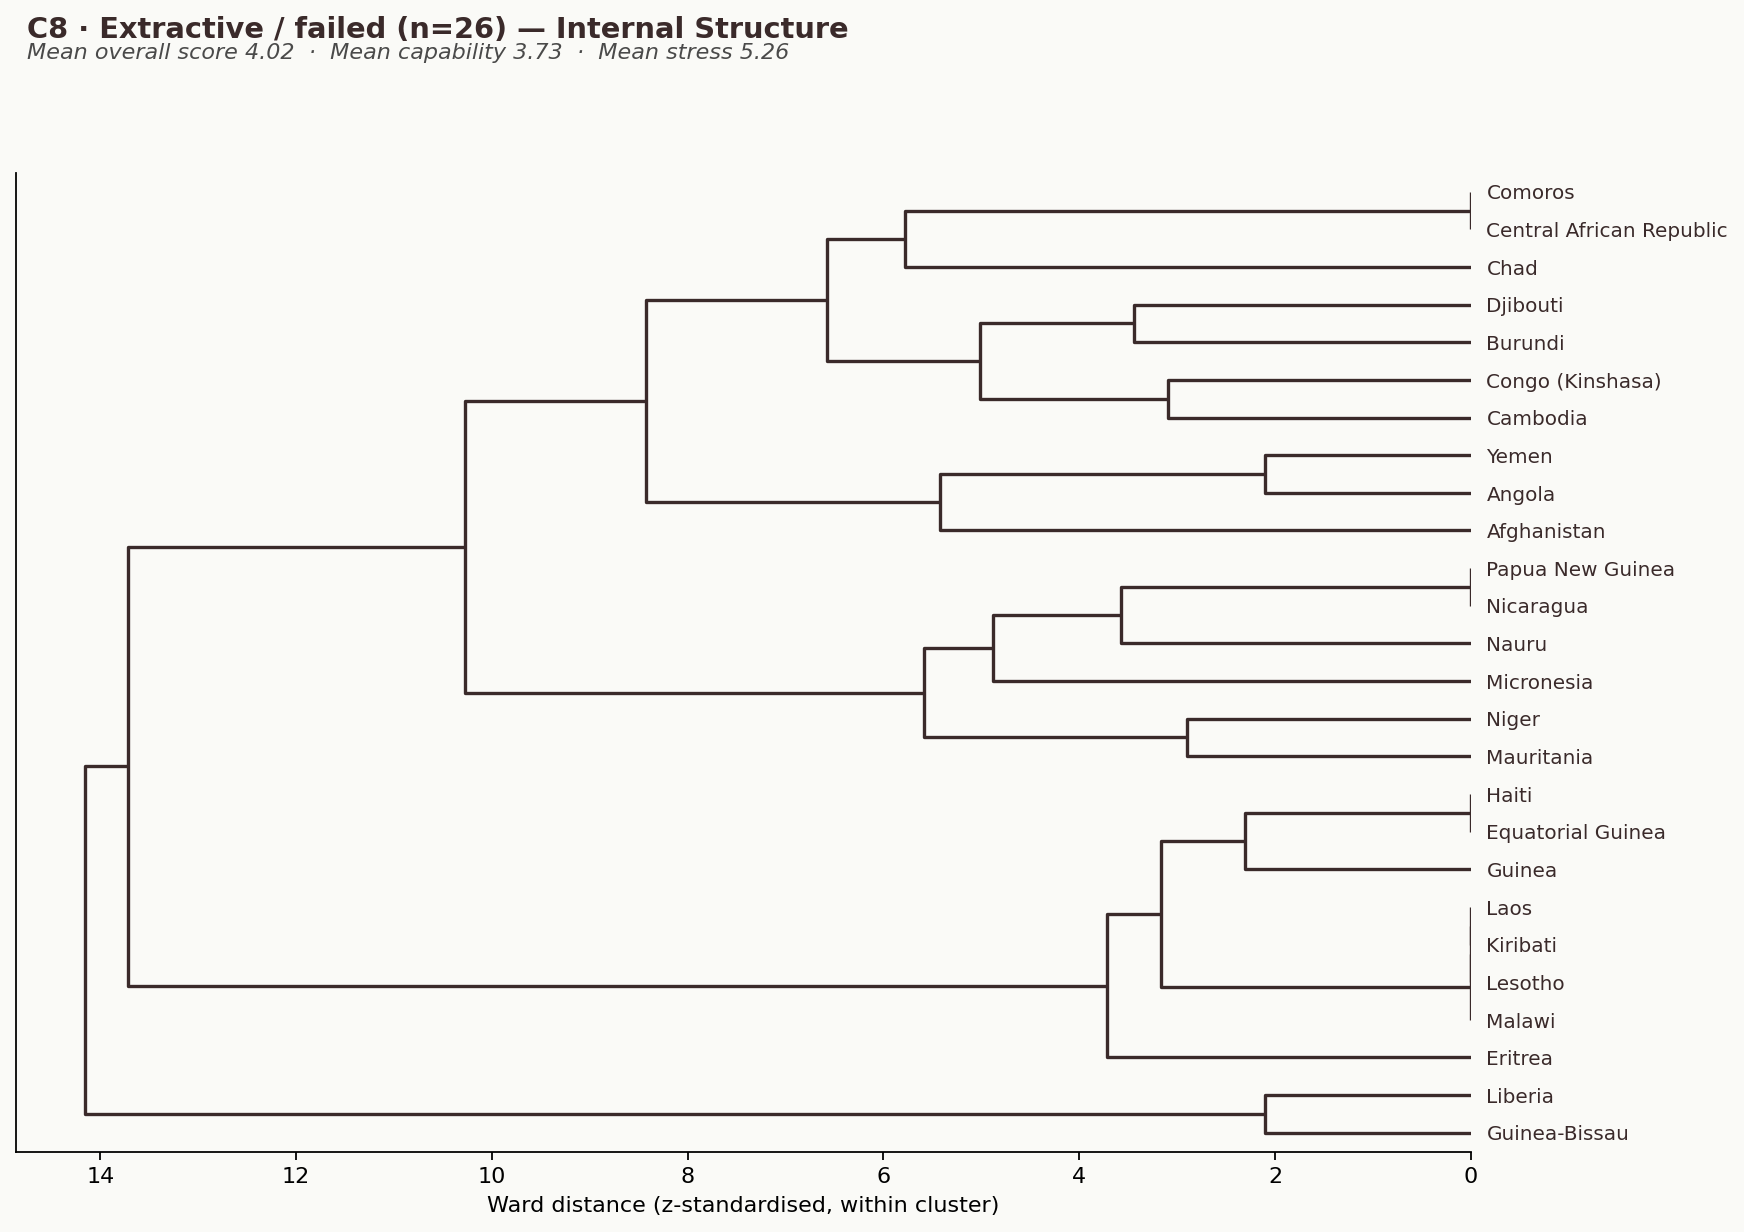
\includegraphics[width=\textwidth, height=0.82\textheight, keepaspectratio]{dendro_C8_Extractive__failed}
  \caption{\textbf{C8 $\cdot$ Extractive / failed ($n=26$) --- Internal Structure.} Mean overall score 4.02 $\cdot$ Mean capability 3.73 $\cdot$ Mean stress 5.26.}
  \label{fig:c8}
\end{figure}

\newpage
\vspace*{\fill}
\noindent\rule{\textwidth}{0.4pt}
\begin{center}
\small\color{gray}
Draft v3 $\cdot$ May 2026 $\cdot$ Australian English $\cdot$ Figures embedded \\
Reproducibility: \href{https://github.com/KaliBond/wintermute}{github.com/KaliBond/wintermute}
\end{center}
\vspace*{\fill}

\end{document}
